%% ============================================================
%% Food Security Risk Assessment: A Review of GA-ANN and Fuzzy
%% Logic Techniques in Intelligent Systems
%%
%% LaTeX manuscript prepared for submission to
%% Applied Soft Computing (Elsevier), using the elsarticle class
%% and the elsarticle-num (numbered / Vancouver-style) reference
%% style required by the journal's Guide for Authors.
%% ============================================================

\documentclass[preprint,12pt]{elsarticle}
\usepackage[utf8]{inputenc}
\usepackage[T1]{fontenc}
\usepackage{amssymb}
\usepackage{amsmath}
\usepackage{graphicx}
\usepackage{booktabs}
\usepackage{array}
\usepackage{longtable}
\usepackage{url}
\usepackage{hyperref}
\usepackage{seqsplit}
\renewcommand{\topfraction}{0.9}
\renewcommand{\floatpagefraction}{0.8}
\setcounter{topnumber}{2}
\setcounter{totalnumber}{4}

\journal{Applied Soft Computing}

\begin{document}
	
	\begin{frontmatter}
		
		\title{Food Security Risk Assessment: A Review of GA-ANN and Fuzzy Logic Techniques in Intelligent Systems}
		
		\author[unikl]{Sha'elah Mohd Safri}
		
		\author[unikl]{Muhd Khairulzaman Abd Kadir\corref{cor1}}
		\ead{khairulzaman@unikl.edu.my}
		
		\author[uca]{Giovanni Honakoko}
		
		\address[unikl]{Electronics \& Electrical Engineering Technologies, Universiti Kuala Lumpur British Malaysian Institute (UniKL BMI)}
		\address[uca]{Polytech Nice Sophia, Universit\'e C\^ote d'Azur}
		
		\cortext[cor1]{Corresponding author}
		
		\begin{abstract}
			Food security risk assessment evaluates risks to food availability, accessibility, and economic stability by rating the likelihood and severity of adverse events, using indicators such as crop yield, climate variability, and economic growth. This review examines the integration of Genetic Algorithm-Artificial Neural Networks (GA-ANN) and Fuzzy Logic (FL) in food security risk assessment, aiming to propose an integrated GA-ANN-Fuzzy Logic framework enhanced by big data protocols for more comprehensive analysis, better prediction, and more proactive prevention of food security risk. GA-ANN and FL are complementary intelligent-system techniques: the genetic algorithm improves the neural network by identifying the most relevant food security features and independently optimizing parameter values, increasing prediction accuracy, while the ANN identifies patterns and forecasts factors such as crop yield, economic conditions, and supply chain integrity. Fuzzy logic complements both by transforming uncertain information into fuzzy risk categories (e.g., low, moderate, or high risk). To corroborate this potential, the review highlights a fuzzy logic framework that models real-world distribution logistics; by effectively handling imprecise data, the system achieves 90\% classification accuracy, outperforming traditional food security risk models across multiple strategies. By analyzing the integration of these intelligent techniques, the paper provides a roadmap for developing more accurate, interpretable, and scalable food security risk assessment systems.
			
		\end{abstract}
		
		
		
		\begin{graphicalabstract}
			\centering
			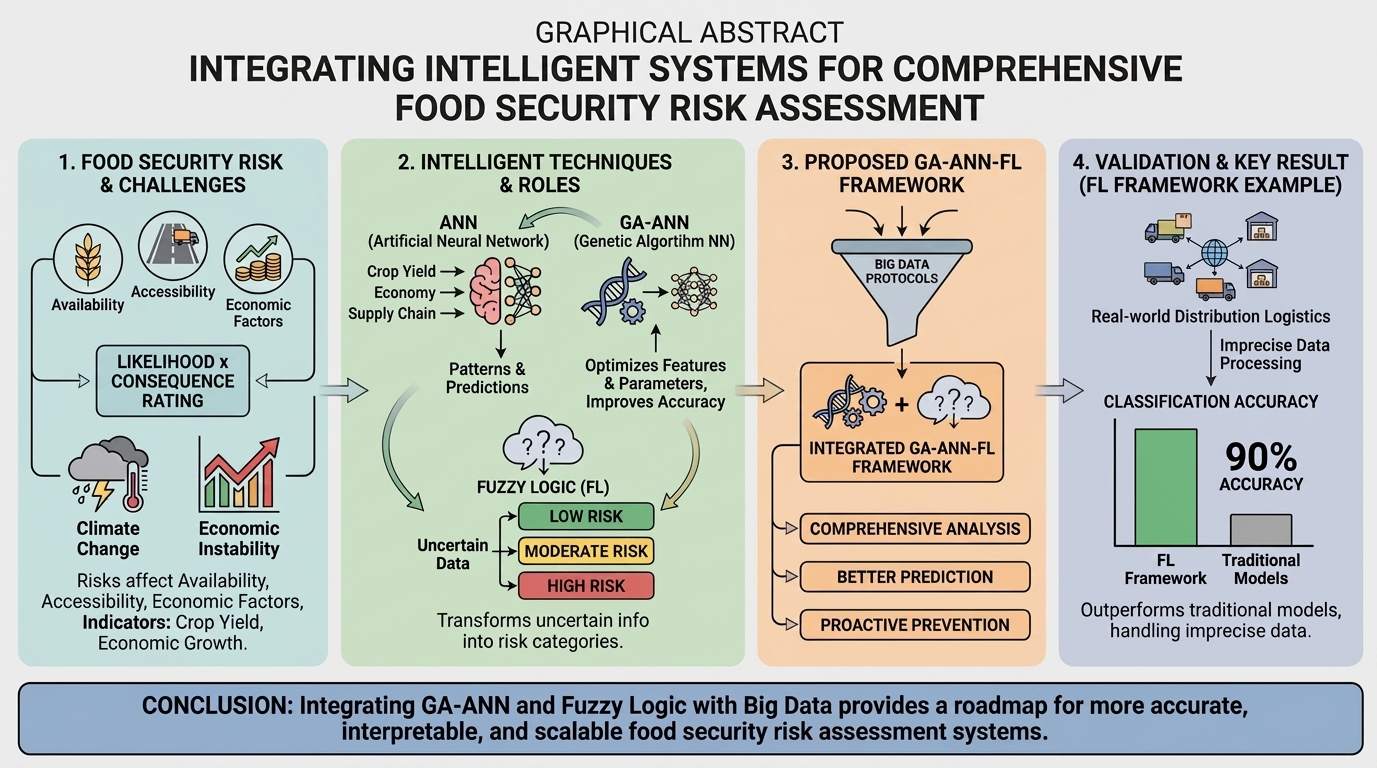
\includegraphics[width=\linewidth,height=0.45\textheight]{figures/graphical_abstract.jpg}
		\end{graphicalabstract}
		
		
		
		\begin{highlights}
			\item Reviews GA-ANN and fuzzy logic synergy for food security risk assessment
			\item Identify 20 key challenges across data, modeling, and system deployment
			\item Highlights the need for climate-resilient and interpretable AI models
			\item Maps a future roadmap for scalable, real-time decision support systems
		\end{highlights}
		
		
		\begin{keyword}
			Food security \sep
			Risk assessment \sep
			Artificial Neural Networks \sep
			Genetic Algorithms \sep
			Fuzzy logic \sep
			Decision support systems
		\end{keyword}
		
	\end{frontmatter}
	
	
	
	\section{Introduction}
	
	Food security remains one of the most pressing global challenges in the
	21st century, exacerbated by climate change, population growth, resource
	constraints, and socio-political instability. Ensuring stable access to
	sufficient, safe, and nutritious food has become a central concern for
	policymakers, researchers, and agricultural stakeholders worldwide.
	Traditional assessment methods, while foundational, often fall short in
	capturing the complex and dynamic nature of food security risks in
	modern ecosystems. As a result, there is growing interest in integrating
	computational intelligence, machine learning (ML), and artificial
	intelligence (AI) techniques to enhance the accuracy, responsiveness,
	and scalability of food security risk assessments.
	
	Food security risk assessment aims to identify and quantify the
	likelihood and severity of threats that compromise food supply chains.
	Traditional methods based on expert judgment, statistical modeling, and
	rule-based systems have been limited by subjectivity, static
	assumptions, and difficulty handling uncertainty \cite{ref1}. Consequently,
	intelligent techniques such as Artificial Neural Networks (ANN), Genetic
	Algorithms (GA), and Fuzzy Logic (FL) have gained traction due to their
	adaptability, learning capacity, and ability to manage nonlinearity and
	imprecision.
	
	ANNs are particularly effective at detecting hidden patterns and
	nonlinear relationships in agricultural and economic datasets, enabling
	them to forecast parameters such as crop yield, market volatility, or
	food supply trends \cite{ref2}. However, standard ANN models often suffer from
	local minima issues and slow convergence. To overcome this, hybrid
	models like GA-ANN combine the optimization power of genetic algorithms
	with the learning capacity of neural networks, improving both prediction
	accuracy and model robustness \cite{ref3}.
	
	Fuzzy Logic, by contrast, excels in modeling linguistic and uncertain
	data. It transforms vague inputs such as ``low yield'' or ``high risk'' into
	numerical outputs, making it ideal for scenarios where crisp
	classification is impractical. FL-based systems have been applied
	successfully to evaluate food security levels, integrating multiple
	dimensions such as production output, economic indicators, and
	policy-related data \cite{ref4}.
	
	As big data technologies evolve, risk assessment systems increasingly
	leverage large, unstructured, and often unlabeled datasets from
	satellite imagery, IoT devices, and national food registries. In
	response, recent research has proposed autonomous decision support
	systems that combine unsupervised learning, clustering, and fuzzy
	inference to handle uncertainty and scale \cite{ref5}. These models achieve
	high performance even under data ambiguity, outperforming traditional
	machine learning models in scenarios with incomplete or noisy inputs.
	
	In a notable study, a fuzzy decision support system utilizing 500,000 UK
	driving records across two decades demonstrated consistent
	classification of food-related risks using optimistic, pessimistic, and
	neutral strategies \cite{ref5}. Similarly, applications of backpropagation
	(BP) neural networks have been explored in early warning systems for
	national food security in China, offering dynamic, data-driven models
	for proactive intervention and policymaking \cite{ref6}. Other studies have
	shown the efficacy of multi-model fusion techniques in specific
	agricultural domains, such as rice risk assessment, by integrating
	clustering algorithms, expert-based weighting, and high-dimensional
	machine learning \cite{ref1}.
	
	Beyond technical advances, food security analysis is complicated by the
	fact that risks are inherently multi-dimensional, spanning
	environmental, social, political, and economic domains. Multi-criteria
	decision-making (MCDM) methods integrated with fuzzy logic allow
	researchers to weigh trade-offs between conflicting factors, offering
	more holistic decision frameworks in uncertain contexts \cite{ref94}. Climate
	variability further amplifies these complexities, as shifting rainfall
	patterns and temperature extremes introduce major uncertainties in crop
	yields and food supply. Hybrid GA-ANN models have shown promise in
	predicting such yield fluctuations more reliably than traditional
	regression methods, providing valuable foresight for adaptive planning
	
	\cite{ref95}.
	
	The integration of IoT devices and satellite remote sensing into food
	security monitoring is another emerging direction. These systems
	generate vast, real-time datasets on soil health, crop growth, and
	supply logistics. When combined with fuzzy logic and ANN frameworks,
	they enable proactive monitoring of agricultural performance and early
	identification of risks such as drought, pest outbreaks, or supply chain
	disruptions \cite{ref96}. However, such data sources are often sparse or
	incomplete. Hybrid GA-ANN approaches, especially when coupled with
	robust imputation techniques, have demonstrated resilience against
	missing data, allowing for reliable predictions even under fragmented
	information \cite{ref97}.
	
	A growing body of research emphasizes the role of intelligent
	early-warning systems in food security. By combining fuzzy-based
	reasoning with ANN prediction engines, these systems can detect weak
	signals of disruption and provide actionable alerts to policymakers,
	reducing the likelihood of crises escalating unchecked \cite{ref98}. To
	achieve this at scale, GA-ANN models have increasingly been embedded
	into cloud-based infrastructures, enabling distributed processing and
	real-time analysis across diverse geographic regions \cite{ref99}.
	
	
	
	\begin{figure}[tp]
		\centering
		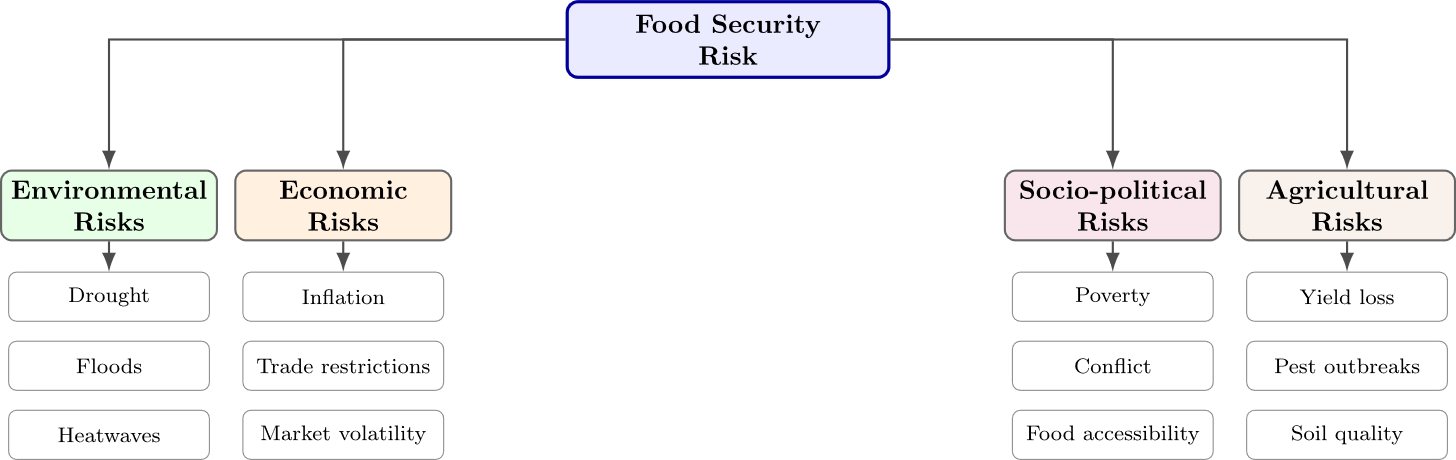
\includegraphics[width=1\linewidth,height=1\textheight,keepaspectratio]{figures/fig01.png}
		\caption{Major Drivers of Food Security Risk}
		\label{fig:fig01}
	\end{figure}
	
	Food security is not only determined by
	physical availability but also by socio-economic conditions. Indicators
	such as household income, inflation, and trade restrictions play a
	pivotal role in accessibility. Fuzzy-based systems are particularly
	effective at translating ambiguous socio-economic indicators into
	structured inputs for ANN-driven predictions, enhancing the reliability
	of food security risk assessments \cite{ref100}. Moreover, policy
	interventions such as subsidies or import regulations have long-term
	consequences for supply-demand balance. Hybrid GA-ANN and FL systems can
	simulate alternative policy scenarios, supporting more informed and
	forward-looking decision-making \cite{ref101}. Food security is shaped by a
	complex combination of environmental, economic, social, political, and
	agricultural factors; rather than acting independently, these drivers
	often interact and reinforce one another, influencing food availability,
	access, utilization, and stability. To provide a structured overview of
	these relationships, the following figure summarizes the principal
	sources of food security risk examined in this review.
	
	Environmental disruptions such as droughts, floods, and climate
	variability directly affect agricultural productivity, while economic
	and governance-related factors influence access to food and market
	functioning. Recognizing these interdependencies is essential for the
	development of intelligent assessment systems capable of capturing the
	complexity of real-world food security conditions. Furthermore, the
	adaptability of computational systems to local contexts remains
	critical. Food security risks differ substantially between developed and
	developing countries, as well as across agro-ecological zones. Localized
	fuzzy inference systems optimized by GA-ANN models have demonstrated
	effectiveness in smallholder farming contexts, where food security risks
	are often most acute \cite{ref102}. Moving forward, the convergence of GA-ANN,
	FL, and big-data-driven protocols into unified frameworks represents a
	promising frontier. These integrated systems can simultaneously manage
	uncertainty, optimize performance, and provide interpretable insights,
	thus offering a comprehensive foundation for data-driven policy and
	practice in food security risk management \cite{ref10}.
	
	This review paper seeks to comprehensively evaluate the role of GA-ANN
	and Fuzzy Logic based systems in food security risk assessment. Drawing
	from six foundational studies, it identifies their individual strengths,
	synergy, and applicability in real-world settings. Ultimately, the paper
	aims to outline a conceptual roadmap for integrating GA-ANN and FL into
	a unified framework, enhanced by big data protocols, to improve
	prediction accuracy, resilience, and policy responsiveness in food
	security management.
	
	\section{Research Background}
	
	The study of food security risk assessment has evolved alongside
	advances in artificial intelligence, particularly in fields that require
	modeling of complex, nonlinear, and uncertain systems. Traditionally,
	risk assessments in food systems relied heavily on deterministic or
	semiquantitative models that incorporated statistical thresholds and
	expert judgment to define vulnerability, exposure, and impact across
	supply chains \cite{ref8}. However, with the growing volume, velocity, and
	variety of agricultural and environmental data, conventional models have
	shown limitations in scalability, adaptability, and interpretability.
	
	Artificial Neural Networks (ANNs) have emerged as robust tools for
	learning complex patterns from large, high-dimensional datasets. In
	agriculture, they have been extensively used for yield prediction, soil
	analysis, irrigation modeling, and post-harvest quality control \cite{ref2}.
	Despite their effectiveness, ANNs are often challenged by issues of slow
	convergence, local minima entrapment, and sensitivity to initialization
	parameters. To mitigate these drawbacks, researchers have increasingly
	employed Genetic Algorithms (GA) to optimize the structure and weight
	parameters of ANN models, resulting in GA-ANN hybrids that outperform
	standalone neural networks in both accuracy and generalization \cite{ref3},
	\cite{ref1}.
	
	In parallel, Fuzzy Logic (FL) systems have gained attention for their
	ability to model human-like reasoning under uncertainty. Unlike binary
	logic systems, FL operates on degrees of truth, which makes it suitable
	for handling linguistic variables (e.g., ``low yield'', ``moderate risk'')
	and vague data a common characteristic in food security domains where
	data may be imprecise, incomplete, or subjective \cite{ref4}. Fuzzy logic has
	been employed to assess food security at both micro (crop-level) and
	macro (national policy) levels, where economic indicators, production
	data, and climate conditions interact in unpredictable ways \cite{ref5}.
	
	The convergence of these techniques has led to the development of
	integrated models such as Genetic Neuro-Fuzzy (GNF) systems, which
	combine the learning capability of ANNs, the global optimization ability
	of GA, and the uncertainty modeling strength of FL. These systems aim to
	support real-time decision-making in dynamic environments by producing
	interpretable outputs with high prediction accuracy \cite{ref1}. For instance,
	in a notable application, a fuzzy logic-based framework was used to
	classify food security risk using a dataset of over 500,000 driving
	journeys as a proxy for economic activity and distribution logistics,
	demonstrating an accuracy of 90\% across pessimistic, neutral, and
	optimistic scenarios \cite{ref6}.
	
	On a national scale, the application of backpropagation (BP) neural
	networks for early warning systems has been explored in China, where
	food security risks were classified into multiple levels (no warning,
	light warning, moderate warning, and heavy warning) based on indicators
	such as grain output, ecological conditions, and trade dynamics \cite{ref6}.
	The model combined principal component analysis (PCA) and analytic
	hierarchy process (AHP) to construct a multidimensional risk index,
	validated against data from 2000 to 2019.
	
	Additionally, fusion models that integrate unsupervised clustering,
	expert knowledge weighting such as AHP, DEMATEL and ensemble machine
	learning have shown promising results in domain-specific assessments
	such as rice production risk across 31 provinces in China. These models
	can handle high-dimensional hazard detection data and yield
	classification accuracy exceeding 99\%, validating their reliability for
	regulatory and policy applications \cite{ref5}.
	
	
	
	\begin{figure}[tp]
		\centering
		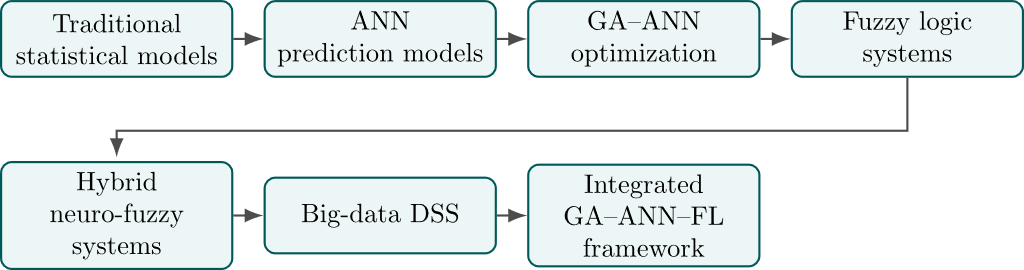
\includegraphics[width=1\linewidth,height=1\textheight,keepaspectratio]{figures/fig02.png}
		\caption{Evolution of AI-Based Food Security Assessment Approaches}
		\label{fig:fig02}
	\end{figure}
	
	The combination of GA-ANN and FL
	techniques within food security modeling is not merely additive it is
	synergistic. GA improves the adaptability of ANN, while FL adds
	interpretability and robustness in the face of ambiguous inputs.
	Together, they provide a foundation for the next generation food
	security risk assessment systems that are both precise and explainable.
	This integrated approach not only addresses prediction tasks but also
	supports strategic decisions for early warning systems, sustainable
	planning, and supply chain optimization. Research on food security
	assessment has evolved considerably over the past decades. Early studies
	relied primarily on statistical and econometric techniques, whereas more
	recent work has incorporated machine learning, optimization methods, and
	hybrid intelligent systems. Figure 2 outlines the main stages of this
	methodological evolution.
	
	\section{Related Studies}
	
	
	
	\begin{figure}[tp]
		\centering
		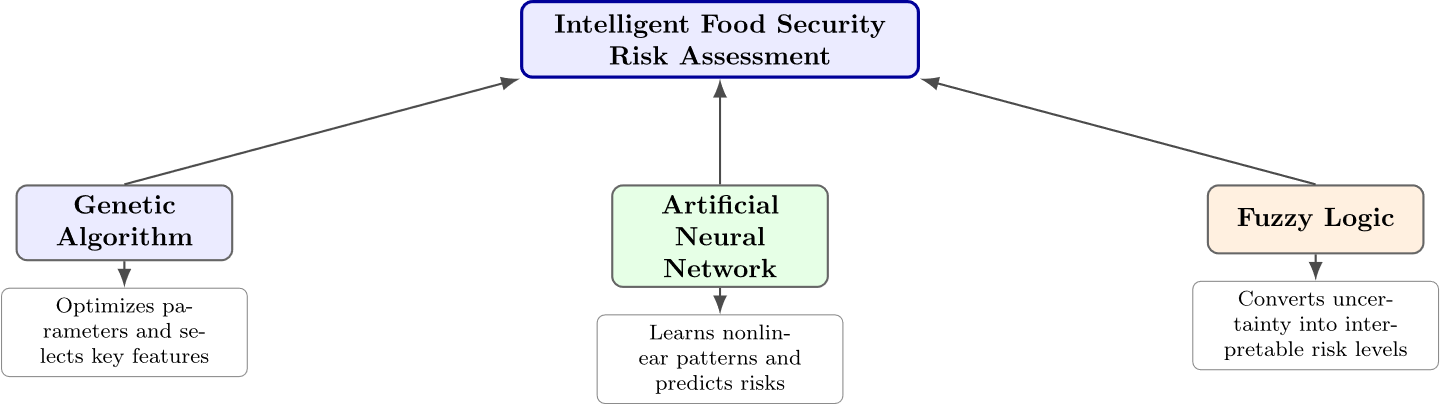
\includegraphics[width=1\linewidth,height=1\textheight,keepaspectratio]{figures/fig03.png}
		\caption{Functional Roles of GA, ANN and Fuzzy Logic in Food Security Assessment}
		\label{fig:fig03}
	\end{figure}
	
	Research on food security risk assessment
	has advanced significantly in recent years, driven by the integration of
	machine learning, fuzzy logic, hybrid soft computing, and
	big-data-driven decision support systems. The following review clusters
	relevant studies into four main thematic areas: neural-based approaches,
	fuzzy and hybrid methods, big-data-driven decision support, and early
	warning/ecological frameworks. The intelligent approaches reviewed in
	this study rely on several complementary computational techniques.
	Before reviewing individual contributions, it is useful to distinguish
	the specific role that Genetic Algorithms, Artificial Neural Networks,
	and Fuzzy Logic typically play within food security applications.
	
	
	
	\begin{figure}[tp]
		\centering
		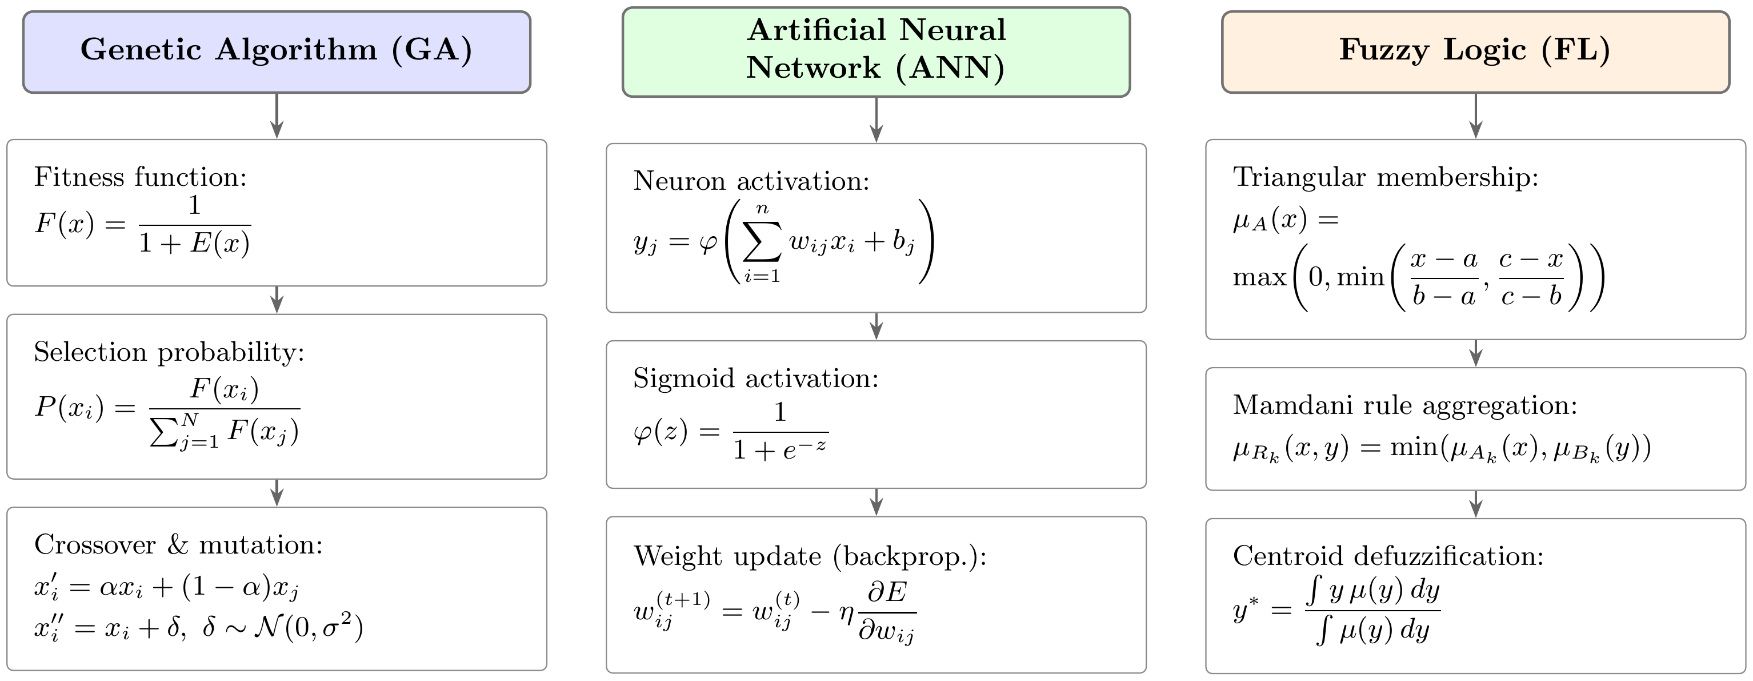
\includegraphics[width=1\linewidth,height=1\textheight,keepaspectratio]{figures/fig04.png}
		\caption{Mathematical Formulation of GA, ANN, and Fuzzy Logic Components}
		\label{fig:fig04}
	\end{figure}
	
	
	
	
	\subsection{Neural-based Approaches}
	
	Artificial neural networks and related machine-learning methods have
	been widely applied to food security risk assessment. The study in
	\cite{ref12} proposed to fuse multiple machine-learning models for rice
	security assessment, achieving improved detection accuracy across
	heterogeneous datasets. Similarly, \cite{ref13} proposed to optimize banana
	yield in greenhouse environments through a combination of generalized
	regression neural networks (GRNN) and genetic algorithms for nutrient
	optimization. Predictive modeling approaches have also been extended to
	food safety, such as \cite{ref7}, which applied tree-based ML algorithms to
	predict \emph{Salmonella} outbreaks, and \cite{ref32} and \cite{ref33}, which forecast
	acute food insecurity by integrating high-frequency health and
	environmental indicators. Ensemble methods such as Bayesian model
	averaging \cite{ref19} and hybrid random forest--MLP models \cite{ref27} have been
	proposed to enhance ecological security evaluations in grain-producing
	areas. In addition, \cite{ref20} introduced a hybrid GA--fuzzy neural model
	tailored for crop yield prediction, highlighting the potential of
	combining neural inference with evolutionary optimization. Similarly,
	\cite{ref21} demonstrated the application of ANN-based frameworks for early
	detection of food insecurity at regional scales, reinforcing the value
	of neural approaches in anticipatory risk management.
	\smallskip
	
	
	More recent efforts extend neural-based forecasting to global markets
	\cite{ref51} applied recurrent neural networks to predict staple food price
	volatility under climate stress, while \cite{ref52} used convolutional neural
	networks (CNNs) to classify crop stress signals from satellite imagery,
	improving early identification of yield losses. Likewise, \cite{ref53}
	developed a deep reinforcement learning framework to optimize irrigation
	decisions under uncertain rainfall, demonstrating the adaptability of
	neural models to decision-oriented contexts. Across these studies,
	neural-based approaches demonstrate high predictive accuracy, but they
	often face challenges in interpretability
	
	
	\begin{figure}[tp]
		\centering
		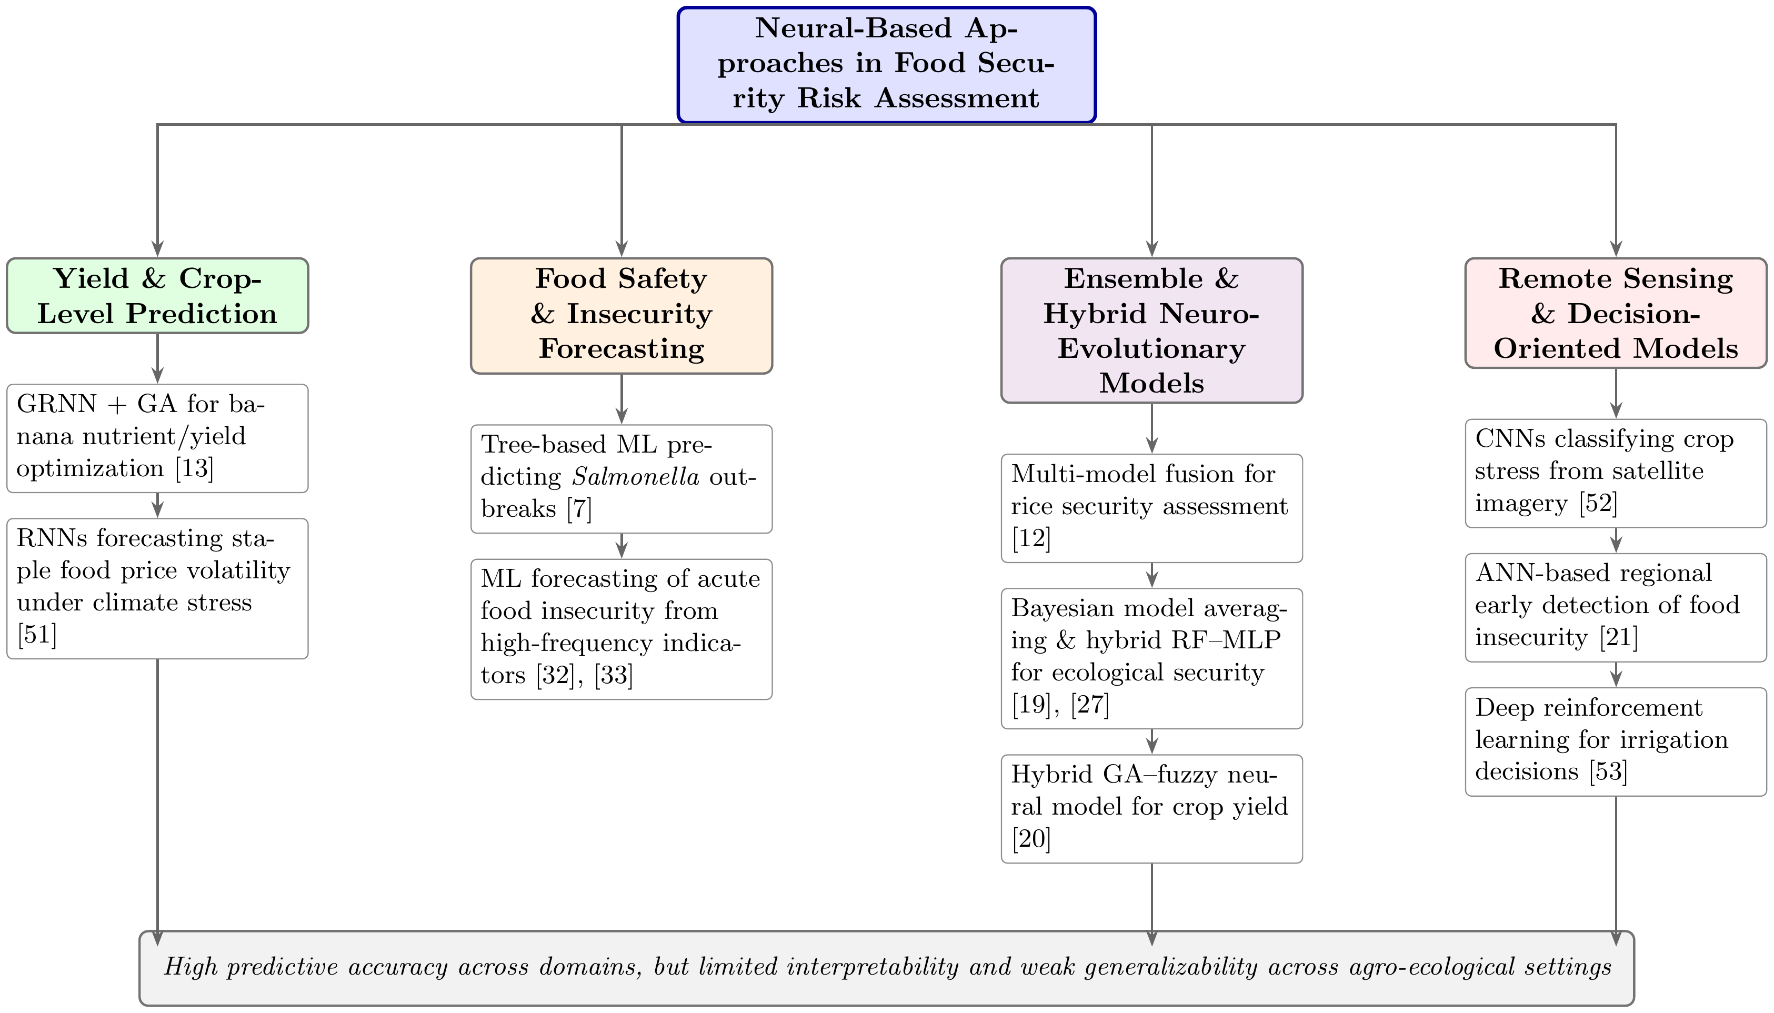
\includegraphics[width=1\linewidth,height=1\textheight,keepaspectratio]{figures/fig05.png}
		\caption{Taxonomy of Neural-Based Approaches in Food Security Risk Assessment}
		\label{fig:fig05}
	\end{figure}
	
	and generalizability across diverse
	agro-ecological settings.
	
	\subsection{Fuzzy and Hybrid Soft-Computing}
	
	Fuzzy systems and hybrid models combining fuzzy logic with neural
	networks or evolutionary algorithms have been applied to address
	uncertainty in food security risk modeling. The study \cite{ref15} proposed a
	Mamdani fuzzy logic system for assessing food security risk levels,
	while \cite{ref14} introduced a hybrid fuzzy-neural approach to reduce
	uncertainty in agricultural predictions. Hybrid optimization techniques
	such as ANFIS combined with multi-objective genetic algorithms \cite{ref22,ref26}
	have been proposed for yield forecasting, while fuzzy-based DSS
	frameworks \cite{ref25,ref36} enable resilient decision making under imprecise
	information. Applications in agricultural supply chains have been a key
	focus \cite{ref37} and \cite{ref38} applied fuzzy TOPSIS and fuzzy-AHP methods to
	evaluate risks in financing and rice supply chains, respectively, while
	\cite{ref40} used spherical fuzzy AHP to model pandemic-driven disruptions.
	Other works, such as \cite{ref39} and \cite{ref46}, demonstrated hybrid fuzzy
	methods for supply chain performance evaluation, integrating risk
	metrics like time, cost, and quality. Further, \cite{ref54} proposed a
	Z-number fuzzy inference system for food logistics under uncertainty,
	and \cite{ref55} presented a hybrid GA--fuzzy model to optimize fertilizer use
	efficiency across diverse crop systems. Recent innovations also include
	\cite{ref34} and \cite{ref35}, which applied interval type-2 fuzzy logic and
	intuitionistic fuzzy models, respectively, to agricultural
	decision-making under high uncertainty, demonstrating that extended
	fuzzy frameworks can better handle ambiguous and conflicting inputs in
	food system risk scenarios. These approaches highlight the adaptability
	of fuzzy systems for modeling imprecision, but they also require expert
	input, which can introduce subjectivity in risk assessment.
	
	\subsection{Big-Data Driven Decision Support Systems}
	
	The rise of big data has enabled the construction of advanced decision
	support systems (DSS) for food security. The study in \cite{ref17} proposed an
	autonomous fuzzy DSS that integrates multisource big data for risk
	assessment, while \cite{ref18} surveyed Agriculture 4.0 DSS, emphasizing
	ML-enabled farm-level decision support. Studies such as \cite{ref7,ref43,ref44} have
	focused on integrating large heterogeneous datasets, including news
	text, climate indicators, and conflict event data, to predict food
	insecurity. Data harmonization efforts such as the HFID dataset \cite{ref42}
	and explainable AI frameworks \cite{ref24} demonstrate progress toward
	transparent and scalable monitoring tools. Meanwhile, organizations such
	as WFP have explored machine-learning-driven early warning platforms
	\cite{ref45}, while \cite{ref41} examined socio-economic drivers of food insecurity
	using ML on survey data. Additional advances include \cite{ref56}, which
	proposed federated learning architectures for cross-country food risk
	analysis, and \cite{ref57}, which integrated graph neural networks with
	big-data pipelines to map cascading food supply disruptions. Similarly,
	\cite{ref58} developed a blockchain-enabled DSS for agricultural trade risk
	monitoring, showing the potential for coupling data integrity with
	AI-driven prediction. Together, these studies underline the potential of
	big-data DSS in providing real-time, data-driven insights for proactive
	interventions.
	
	\subsection{Early Warning Systems and Ecological Risk Frameworks}
	
	
	
	\begin{figure}[tp]
		\centering
		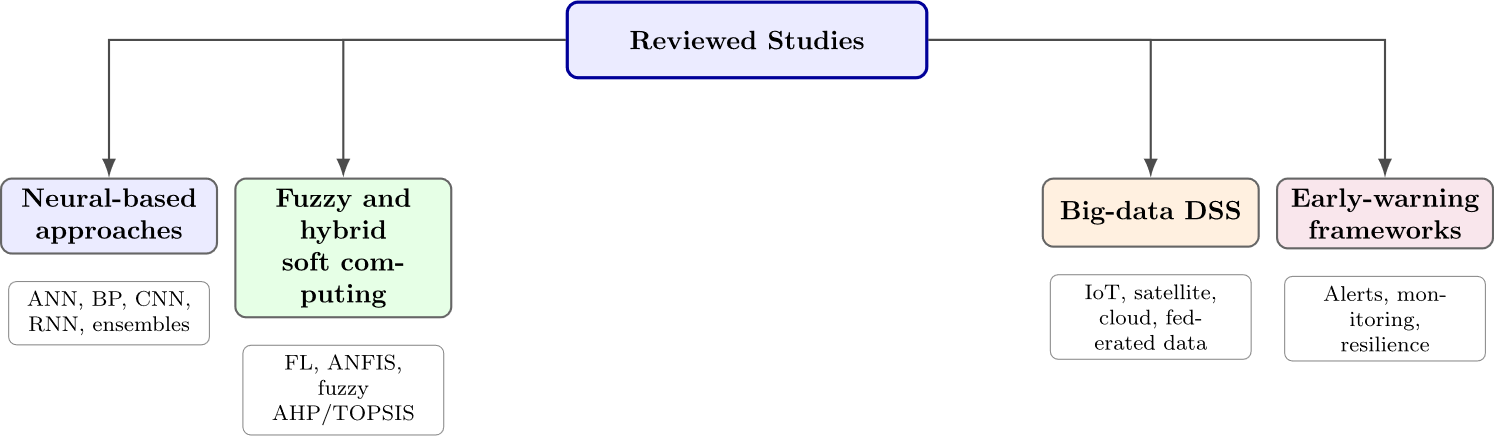
\includegraphics[width=1\linewidth,height=1\textheight,keepaspectratio]{figures/fig06.png}
		\caption{Classification of Reviewed Studies}
		\label{fig:fig06}
	\end{figure}
	
	Early warning systems (EWS) are critical
	for mitigating food security risks before crises escalate. Neural and
	hybrid models have been widely adopted in this space \cite{ref16} used a BP
	neural network combined with AHP for China's food security early
	warning, while \cite{ref28} proposed a 3D visualization platform integrating
	GA-BP models for dynamic monitoring. Similarly, \cite{ref23} and \cite{ref29}
	improved BP and anomaly detection methods for food safety surveillance.
	Ecological and supply-chain risk frameworks complement these EWS.
	Studies such as \cite{ref30} and \cite{ref48} assessed ecological security in
	grain-producing regions, while \cite{ref47} applied fuzzy logic to supply
	chain risk in perishable foods. Fuzzy FMEA models \cite{ref49} and real-time
	event-driven fuzzy supply chain monitoring \cite{ref50} illustrate the
	potential for combining classical risk management frameworks with modern
	data streams. More recently, \cite{ref59} applied ensemble anomaly detection
	for locust outbreak monitoring, while \cite{ref60} integrated
	satellite-derived drought indices with fuzzy EWS models for sub-Saharan
	Africa. These works demonstrate strong progress in EWS, but challenges
	remain in ensuring scalability, cross-regional applicability, and
	integration of socioeconomic indicators alongside biophysical data. To
	support a systematic analysis of the literature, the selected studies
	were organized into four thematic categories according to their
	methodological orientation and primary application focus.
	
	
	\subsection{Summary}
	
	Overall, neural-based models excel at prediction accuracy but often lack
	transparency; fuzzy and hybrid systems manage uncertainty effectively
	but can be resource-intensive; big-data DSS platforms offer scale and
	real-time monitoring but face integration challenges; and early warning
	systems combine these approaches but require more cross-disciplinary
	data sources. Future research should focus on hybrid frameworks that
	balance predictive power, interpretability, and practical usability for
	policy and on-farm decision making.
	
	\section{Research Challenge}
	
	Despite significant progress in applying artificial intelligence (AI),
	machine learning (ML), and fuzzy-based approaches to food security risk
	assessment, there are still substantial gaps that hinder their
	large-scale and practical deployment. This section highlights ten key
	challenges, each of which requires further investigation to move from
	theoretical contributions to actionable, policy-driven solutions.
	
	\subsection{Data Quality and Availability}
	
	The foundation of any AI or ML model is data. However, the availability
	of reliable, high-quality datasets remains a significant obstacle.
	Agricultural and food security data are often fragmented, outdated, or
	collected inconsistently across regions. In rice security assessment,
	for example, accurate predictions depend on integrating climatic, soil,
	and socio-economic variables, yet such comprehensive datasets are rarely
	available in low-resource countries \cite{ref61}. The lack of standardization
	in data collection further complicates model training and validation,
	often resulting in biased or underperforming models when applied outside
	of their initial test environment.
	
	\subsection{Data Integration Across Sources}
	
	Beyond data availability, the challenge of combining multiple data
	sources into a coherent framework persists. Food security is influenced
	by a wide array of factors, ranging from crop yield and weather
	conditions to market fluctuations and political stability. Greenhouse
	banana yield prediction, for instance, requires the simultaneous
	collection of nutrients (nitrogen, potassium, magnesium) and
	environmental data \cite{ref62}. Integrating such heterogeneous data streams
	into a unified model is complex, as it demands advanced data fusion
	techniques that can handle temporal, spatial, and contextual
	variability.
	
	\subsection{Model Complexity vs. Interpretability}
	
	One of the paradoxes in food security risk modeling is the trade-off
	between accuracy and interpretability. Hybrid models combining genetic
	algorithms, neural networks, and fuzzy logic can produce highly accurate
	results \cite{ref9}, \cite{ref4}. However, their complexity makes them difficult for
	non-technical stakeholders, such as policymakers or farmers, to
	understand. The ``black box'' nature of neural networks limits their
	transparency, raising concerns about accountability in decision-making.
	For food security to benefit from AI, researchers must develop models
	that are both accurate and interpretable, possibly through explainable
	AI techniques.
	
	\subsection{Scalability for Big Data}
	
	Scalability remains a technical bottleneck. Many AI-driven systems are
	tested on relatively small datasets or in controlled environments, but
	they falter when applied to national or global data flows. With the rise
	of big data sources such as remote sensing imagery, IoT-based farm
	sensors, and large agricultural databases models must be capable of
	handling vast amounts of information in near real-time \cite{ref11}.
	Unfortunately, most current models cannot efficiently process such
	volumes without sacrificing performance or accuracy, limiting their
	applicability in operational food security monitoring systems.
	
	\subsection{Real-Time Decision Support}
	
	Timely intervention is critical in food security, especially when
	responding to emerging threats such as droughts, pest outbreaks, or
	sudden market shifts. However, many existing fuzzy decision support
	systems and neural network frameworks suffer from processing delays
	\cite{ref63}. This latency reduces their usefulness in contexts where rapid
	responses are required to mitigate food crises. Building lightweight,
	real-time algorithms that can provide instant risk assessments remains
	an open challenge, especially in resource-constrained settings where
	computational infrastructure is limited.
	
	\subsection{Regional Adaptability and Transferability}
	
	Most models are designed and tested within specific geographic or
	socio-economic contexts. For example, BP neural networks trained on
	Chinese datasets for early warning systems \cite{ref11} may not generalize
	well to African or Latin American contexts, where agricultural
	practices, climate patterns, and market dynamics differ significantly.
	Adapting models to new regions often requires retraining with local
	data, which may not be available. Developing adaptable and transferable
	frameworks that can learn across domains with minimal reconfiguration
	would enhance the global relevance of food security risk models.
	
	\subsection{Policy Integration and Usability}
	
	Another major limitation lies in the gap between technical advances and
	governance. Policymakers often find AI-driven tools too complex or
	misaligned with policy frameworks \cite{ref4}, \cite{ref63}. Even when models
	identify risks accurately, their outputs may not translate into
	actionable recommendations. For instance, fuzzy models may classify risk
	levels but fail to suggest concrete interventions. Building
	user-friendly interfaces and decision support systems that bridge the
	technical-policy gap is crucial to ensure that computational tools
	contribute meaningfully to governance and resource allocation.
	
	\subsection{Uncertainty Management}
	
	Food systems are inherently uncertain, influenced by unpredictable
	factors such as climate change, global trade disruptions, and social
	unrest. Fuzzy logic has been widely used to capture this uncertainty
	\cite{ref9}, \cite{ref4}, yet its capacity is often limited when dealing with highly
	dynamic, multifactor interactions. Moreover, uncertainty is rarely
	communicated effectively to policymakers or farmers, who need to
	understand the level of confidence associated with each prediction.
	Improving methods to quantify, propagate, and explain uncertainty in
	food security assessments is therefore essential to support informed,
	risk-aware decision-making.
	
	\subsection{Balancing Accuracy with Computational Efficiency}
	
	High-accuracy models such as deep neural networks often come at the cost
	of computational intensity. These models require advanced hardware,
	large-scale storage, and high energy consumption. In developing
	countries where food security risks are most acute such resources are
	frequently unavailable \cite{ref62}, \cite{ref63}. This creates a paradox: the most
	vulnerable regions may not be able to implement the very systems
	designed to protect them. Research must therefore focus on developing
	lightweight models that balance accuracy with efficiency, making them
	accessible and sustainable across diverse contexts.
	
	\subsection{Ethical and Social Acceptance}
	
	Ethical and social issues must not be overlooked. The use of AI in food
	security raises questions about data privacy, fairness, and
	accountability. For example, if models are trained on biased data, they
	may reinforce existing inequalities by prioritizing certain crops or
	regions \cite{ref61}, \cite{ref4}. Additionally, trust is a critical factor:
	stakeholders may resist adopting AI-driven systems if they fear loss of
	control or lack confidence in technology. Addressing these ethical and
	social challenges is necessary to ensure that AI adoption in food
	security is both inclusive and equitable.
	
	\subsection{Climate Change Impacts on Model Reliability}
	
	Climate change is one of the greatest threats to global food security
	because it introduces significant variability and unpredictability into
	agricultural systems. Traditional AI and ML models are often trained on
	historical datasets that assume relatively stable climate conditions.
	
	However, extreme weather events such as floods, droughts, hurricanes,
	and heatwaves are becoming more frequent and intense due to climate
	change \cite{ref84}. These anomalies disrupt crop yields, supply chains, and
	market stability, rendering past trends a poor predictor of future
	risks. For example, a model trained on past rice yield and rainfall data
	may significantly underestimate losses caused by a sudden prolonged
	drought. Furthermore, most food security datasets underrepresent these
	extremes, which leads to biased models that fail in crisis conditions.
	To improve resilience, researchers must integrate climate projection
	models, remote sensing of environmental stressors, and scenario-based
	simulations into food security assessments. This would allow models to
	better account for non-linear, climate-driven disruptions and improve
	their reliability in forecasting under uncertain environmental futures.
	
	
	
	\begin{figure}[t]
		\centering
		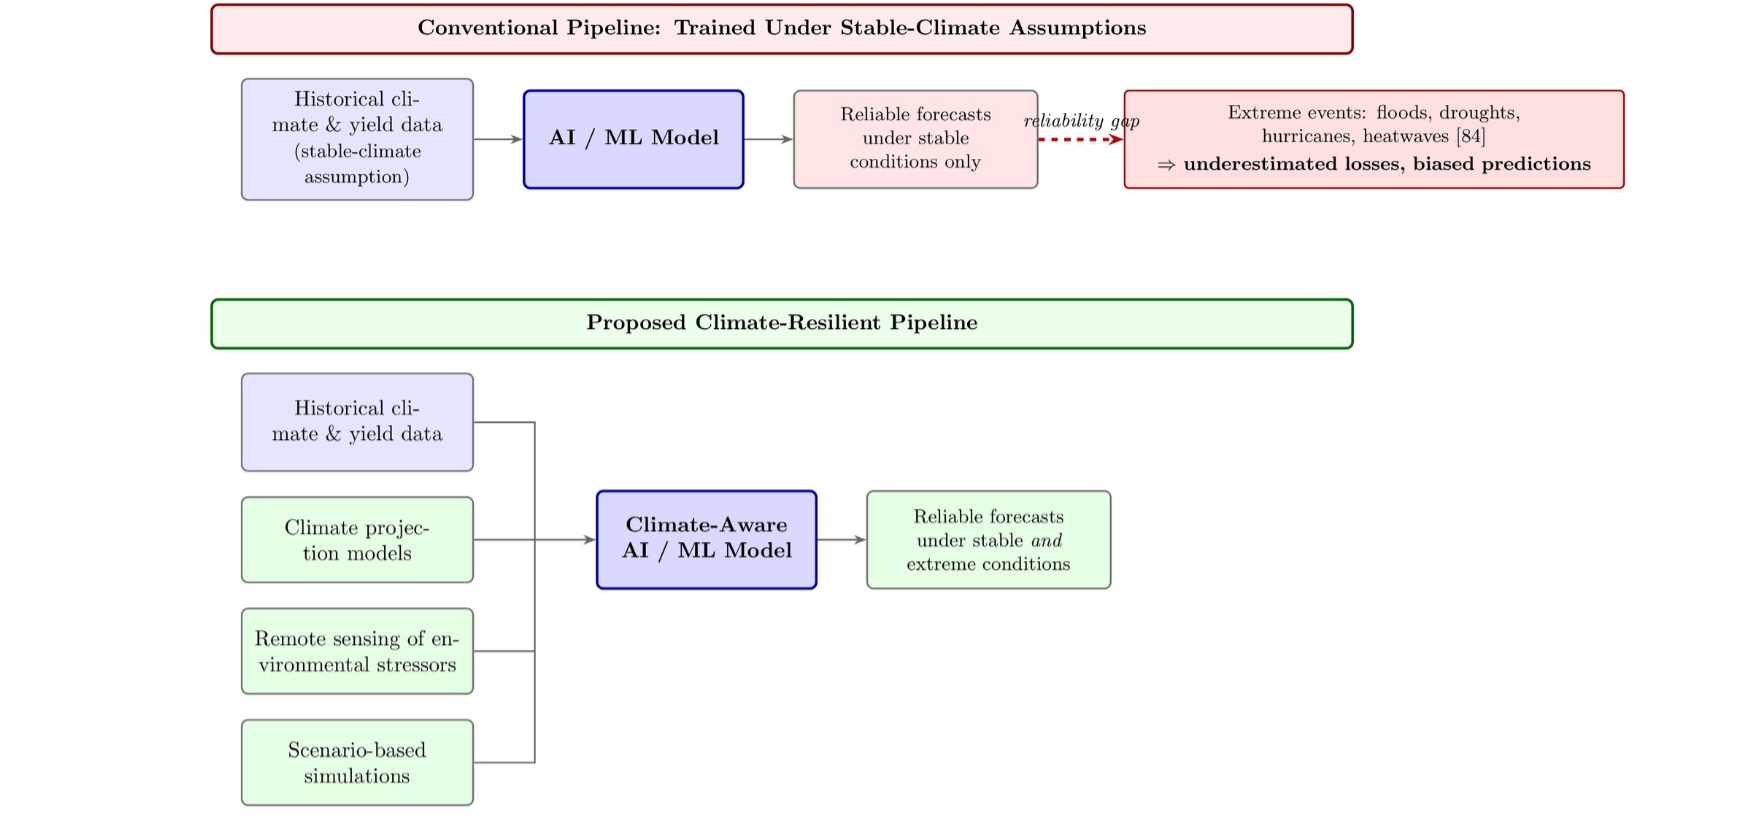
\includegraphics[width=1.05\linewidth,height=0.4\textheight]{figures/fig07.png}
		\caption{Climate Change Impacts on Model Reliability}
		\label{fig:fig07}
	\end{figure}
	
	
	
	Figure 7 contrasts a conventional forecasting pipeline, trained under
	the assumption of stable climate conditions, with the climate-resilient
	pipeline proposed in this review. Because extreme events such as floods,
	droughts, hurricanes, and heatwaves are underrepresented in historical
	training data \cite{ref84}, conventional models develop a growing reliability
	gap and systematically underestimate losses during crisis conditions.
	Integrating climate projection models, remote sensing of environmental
	stressors, and scenario-based simulations alongside historical data
	allows the resulting climate-aware model to remain reliable under both
	stable and extreme conditions.
	
	\subsection{Socio-Economic Factors in Food Security Models}
	
	While technological and environmental factors are central to food
	production, food security also depends heavily on socio-economic
	determinants. Issues such as household income, infrastructure, access to
	markets, food prices, and distribution networks can significantly
	influence food availability and accessibility \cite{ref85}. Many AI-driven
	models disproportionately focus on biophysical variables like soil
	quality, temperature, or rainfall while neglecting socioeconomic
	dimensions. For instance, even when agricultural yields are high,
	vulnerable populations may still face food insecurity if poverty
	prevents them from purchasing adequate food. Similarly, conflict,
	political instability, or trade restrictions can cause severe
	disruptions that models based purely on agricultural production cannot
	capture. Incorporating socio-economic datasets such as household
	surveys, trade indices, and market price fluctuations would make
	predictive systems more holistic and policy relevant. This integration
	would allow researchers to move beyond yield prediction toward
	comprehensive food system risk assessments that address both
	availability and accessibility.
	
	\subsection{Cross-Disciplinary Collaboration Barriers}
	
	Food security is a complex challenge that spans multiple disciplines,
	including agricultural sciences, economics, data science, climatology,
	and policy studies. However, much of the current research is siloed,
	with computer scientists developing advanced algorithms in isolation
	from agricultural experts or social scientists \cite{ref86}. This lack of
	collaboration often produces technically sophisticated models that may
	not align with the realities of farming systems or the needs of
	policymakers. For example, a highly accurate neural network model
	predicting crop yields may not be actionable for farmers if it fails to
	consider practical issues such as irrigation practices, pest management,
	or supply chain constraints. Similarly, policymakers may find outputs
	too technical or abstract to integrate into governance frameworks.
	Bridging these disciplinary divides requires building interdisciplinary
	teams, fostering cross-sector partnerships, and creating collaborative
	platforms where expertise from multiple domains can converge. Only
	through such collaboration can AI-driven models evolve into practical,
	context-aware tools that support sustainable food security strategies.
	
	\subsection{Limited Explainability in Fuzzy-Logic--Based Models}
	
	Fuzzy logic has been widely promoted to model uncertainty in food
	security because it mimics human reasoning and can provide interpretable
	rule-based outputs. However, as fuzzy systems scale up and include
	hundreds or even thousands of fuzzy rules, they themselves can become
	opaque and difficult to interpret \cite{ref87}. For instance, a fuzzy decision
	support system for food insecurity may rely on overlapping rules
	covering climatic, economic, and social dimensions, but the interaction
	among these rules can create outputs that are difficult for stakeholders
	to trace back to specific factors. Policymakers and farmers often
	require simple, actionable insights, not overwhelming rule sets. If
	outputs are too complex, the intended transparency of fuzzy logic may be
	lost, undermining trust and usability. Future research should focus on
	developing methods for simplifying fuzzy models, visualizing outputs in
	user-friendly formats, and integrating explainable AI (XAI) techniques
	that preserve interpretability without sacrificing accuracy.
	
	\subsection{Temporal Data Gaps and Forecasting Limitations}
	
	Food security risk assessment requires not only cross-sectional data but
	also robust temporal datasets that track changes over time.
	Unfortunately, many agricultural datasets are either collected annually
	or irregularly, which severely limits forecasting capacity \cite{ref88}. This
	is particularly problematic for early warning systems, which depend on
	near-real-time data to predict seasonal risks like droughts, pest
	outbreaks, or price shocks. For example, relying solely on annual yield
	statistics does not capture mid-season crop stress caused by erratic
	rainfall or pest infestations. Temporal gaps also limit the ability of
	machine learning models to detect patterns or trends in food security
	risks, resulting in forecasts that may be outdated or incomplete.
	Strengthening data collection through high-frequency monitoring
	technologies such as IoT-based farm sensors, mobile surveys, and remote
	sensing would provide the temporal granularity necessary for dynamic
	forecasting. This would enable proactive responses rather than reactive
	crisis management.
	
	\subsection{Generalization Across Crop Types}
	
	Most AI and ML models developed for food security are highly
	crop-specific, trained and validated on datasets for staple crops such
	as rice, maize, or wheat \cite{ref89}. While these models may perform well
	within a given crop system, their predictive capacity often fails when
	applied to other crops with different physiological and ecological
	characteristics. For instance, a model optimized for rice yield
	prediction may not generalize to banana or cassava due to differences in
	nutrient uptake, disease vulnerability, and growing conditions. This
	crop-specific limitation reduces the utility of AI-based systems in
	regions with diverse agricultural systems. Developing multi-crop models
	or creating transferable frameworks that can adapt across crop types
	with minimal reconfiguration would increase the versatility and
	scalability of food security risk assessments. Such models would also
	support policy frameworks that need to account for the full spectrum of
	agricultural production in each region.
	
	\subsection{Integration with Remote Sensing Technologies}
	
	Remote sensing technologies, particularly satellite imagery, offer a
	powerful means of monitoring agricultural systems at scale, providing
	critical data on vegetation health, soil moisture, and land use \cite{ref90}.
	However, integrating this vast and complex data into AI-driven food
	security assessments remains underdeveloped. Challenges include
	processing high-resolution imagery, aligning satellite data with
	ground-truth observations, and handling noise caused by atmospheric
	conditions or cloud cover. Moreover, most food security models have yet
	to fully exploit the temporal richness of remote sensing data, which can
	provide near-real-time monitoring of crop conditions. Improved
	integration of remote sensing with machine learning models would enhance
	spatial and temporal coverage of food security risk assessments,
	enabling early detection of stressors and more targeted interventions.
	This integration could transform food security monitoring from a largely
	reactive process into a proactive, data-driven system.
	
	\subsection{Resilience to Data Noise and Incompleteness}
	
	Agricultural and food security datasets are frequently noisy,
	incomplete, or inconsistent. Missing values may occur due to logistical
	challenges in data collection, while noise can arise from errors in
	manual surveys, faulty sensors, or environmental variability \cite{ref91}.
	Many machine learning algorithms, particularly deep learning models, are
	highly sensitive to such imperfections and may produce unreliable
	predictions when applied to noisy data. This is a major limitation in
	developing countries where data collection infrastructure is weak.
	Current solutions such as data imputation or preprocessing can help, but
	they often introduce additional biases. Research should focus on
	building robust models that are resilient to imperfect data, capable of
	learning from incomplete information, and able to quantify uncertainty
	arising from noise. Such resilience is critical for ensuring that food
	security risk assessments remain reliable in real-world,
	resource-limited contexts.
	
	\subsection{Lack of Benchmark Datasets and Evaluation Standards}
	
	Unlike fields such as computer vision or natural language processing,
	where benchmark datasets like ImageNet or GLUE exist, food security
	research lacks standardized datasets and evaluation frameworks \cite{ref92}.
	This absence makes it difficult to compare model performance across
	studies or replicate findings, slowing down scientific progress. For
	instance, one study may evaluate food security risk using yield and
	rainfall data, while another uses socio-economic indicators, making
	direct comparisons nearly impossible. Establishing benchmark datasets
	with standardized features and evaluation protocols would foster
	transparency, reproducibility, and innovation in the field. Such
	benchmarks would also create a common ground for interdisciplinary
	collaboration, helping researchers align their efforts toward shared
	objectives.
	
	\subsection{Adoption Barriers in Low-Income Countries}
	
	
	
	\begin{figure}[tp]
		\centering
		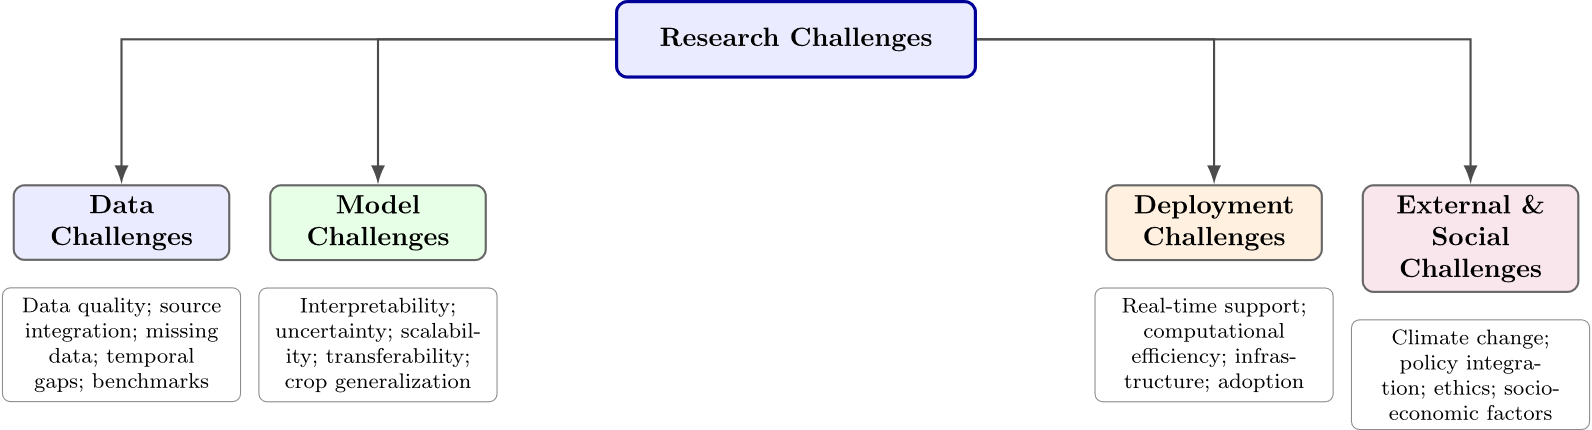
\includegraphics[width=1\linewidth,height=1\textheight,keepaspectratio]{figures/fig08.png}
		\caption{Taxonomy of research challenges in food security risk assessment, categorized by data, model, deployment, and socio-economic dimensions}
		\label{fig:fig08}
	\end{figure}
	
	Even when advanced AI-based systems for
	food security risk assessment exist, their adoption in low-income
	countries remains limited due to a variety of barriers \cite{ref93}. These
	include weak digital infrastructure, low computational capacity, lack of
	technical expertise, and institutional resistance to change.
	Furthermore, vulnerable populations often have low levels of digital
	literacy, limiting their ability to use AI-driven decision support
	systems. This creates a paradox the region most vulnerable to food
	insecurity is often the least equipped to benefit from cutting-edge
	solutions. Overcoming these adoption barriers requires not only
	developing lightweight, low-cost technologies but also investing in
	capacity building, institutional partnerships, and inclusive governance
	frameworks. Research should therefore shift toward implementation
	strategies that are tailored to local contexts, ensuring that
	technological innovations are both accessible and sustainable. Despite
	substantial advances in intelligent food security assessment, a few
	challenges continue to hinder the effectiveness and large-scale adoption
	of existing systems. These challenges extend beyond algorithmic
	performance and involve broader technical, organizational, and societal
	considerations.
	
	\subsection{Summary Table of Research Challenges}
	\small
	\begin{longtable}{@{}p{0.28\linewidth}p{0.10\linewidth}p{0.52\linewidth}@{}}
		\caption{Summary of key research challenges in AI/ML-based food security risk assessment.}
		\label{tab:challenges} \\
		\toprule
		\textbf{Challenge} & \textbf{Ref.} & \textbf{Description} \\
		\midrule
		\endfirsthead
		\multicolumn{3}{c}{\tablename\ \thetable\ -- \textit{continued from previous page}} \\
		\toprule
		\textbf{Challenge} & \textbf{Ref.} & \textbf{Description} \\
		\midrule
		\endhead
		\midrule
		\multicolumn{3}{r}{\textit{continued on next page}} \\
		\endfoot
		\bottomrule
		\endlastfoot
		1. Data Quality and Availability & \cite{ref61} & Lack of reliable, standardized, and comprehensive datasets; fragmented or outdated data hinders robust model development. \\
		2. Data Integration Across Sources & \cite{ref62} & Difficulty in merging heterogeneous sources (climate, soil, socio-economic, IoT, satellite) into a coherent analytical framework. \\
		3. Model Complexity vs. Interpretability & \cite{ref9,ref4} & Hybrid AI models achieve accuracy but act as ``Black boxes,'' limiting transparency and trust for decision-makers. \\
		4. Scalability for Big Data & \cite{ref11} & Many AI systems fail to handle large-scale datasets (IoT, remote sensing) efficiently at national or global levels. \\
		5. Real-Time Decision Support & \cite{ref63} & Existing models suffer from latency, limiting timely interventions during sudden food crises. \\
		6. Regional Adaptability and Transferability & \cite{ref11} & Models trained in specific regions often fail elsewhere; retraining requires local data that may not be available. \\
		7. Policy Integration and Usability & \cite{ref4,ref63} & Outputs are often too technical, lacking actionable insights for policymakers and resource managers. \\
		8. Uncertainty Management & \cite{ref9,ref4} & Current fuzzy and AI methods capture uncertainty only partially; dynamic multi-factor uncertainty is poorly managed. \\
		9. Balancing Accuracy with Computational Efficiency & \cite{ref62,ref63} & High-accuracy models demand advanced infrastructure, which is often unavailable in vulnerable regions. \\
		10. Ethical and Social Acceptance & \cite{ref61,ref4} & Issues of data privacy, fairness, and trust reduce willingness of stakeholders to adopt AI-driven systems. \\
		11. Climate Change Impacts on Model Reliability & \cite{ref84} & AI models trained in historical data struggle to account for climate-driven anomalies like droughts and floods. \\
		12. Socio-Economic Factors in Food Security Models & \cite{ref85} & Many models prioritize biophysical factors while neglecting socio-economic drivers such as poverty and trade access. \\
		13. Cross-Disciplinary Collaboration Barriers & \cite{ref86} & Limited collaboration between computer scientists, agricultural experts, and policymakers reduces real-world usability. \\
		14. Limited Explainability in Fuzzy Logic Models & \cite{ref87} & Large fuzzy systems with complex rule sets become opaque, undermining their intended transparency. \\
		15. Temporal Data Gaps and Forecasting Limitations & \cite{ref88} & Infrequent or annual data collection limits dynamic forecasting for seasonal risks and early warning systems. \\
		16. Generalization Across Crop Types & \cite{ref89} & Most models are crop-specific, reducing their adaptability to diverse agricultural systems. \\
		17. Integrations with Remote Sensing Technologies & \cite{ref90} & Difficulty in incorporating high-resolution satellite imagery into AI models due to noise and alignment issues. \\
		18. Resilience to Data Noise and Incompleteness & \cite{ref91} & Many AI systems are sensitive to missing or noisy agricultural data, reducing reliability in low resource contexts. \\
		19. Lack of Benchmark Datasets and Evaluation Standards & \cite{ref92} & Absence of standard datasets and evaluation protocols hinders reproducibility and model comparison. \\
		20. Adoption Barriers in Low-Income Countries & \cite{ref93} & Weak digital infrastructure, limited technical skills, and institutional barriers slow adoption of AI solutions. \\
		\bottomrule
	\end{longtable}
	
	\section{Future Research Directions}
	
	
	
	\begin{figure}[t]
		\centering
		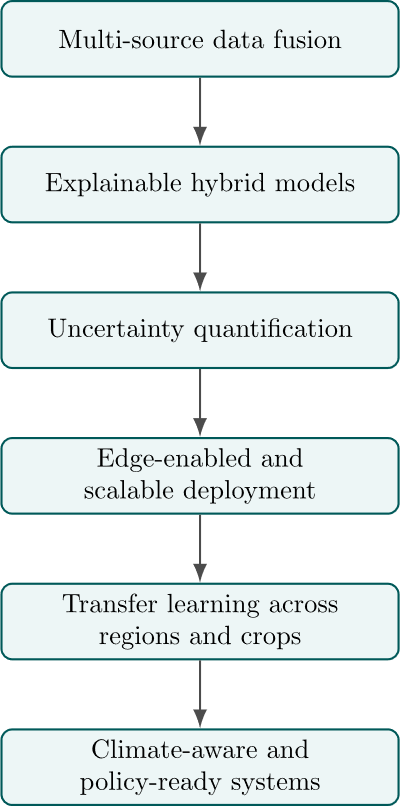
\includegraphics[width=0.85\linewidth,height=0.5\textheight,keepaspectratio]{figures/fig09.png}
		\caption{Future Research Roadmap}
		\label{fig:fig09}
	\end{figure}
	
	The challenges identified throughout
	literature suggest several priorities for future research. There is a
	growing need for assessment systems that are more integrated,
	transparent, scalable, and operationally effective.
	
	\subsection{Advanced Multi-Source Data Fusion}
	
	Food security risk assessment requires data that is often heterogeneous,
	incomplete, or inconsistent across sources. Traditional approaches rely
	on limited datasets, leading to gaps in predictive accuracy and
	coverage. Future work should focus on fusing multi-source datasets such
	as remote sensing imagery, IoT-based soil and weather sensors,
	agricultural management records, market transactions, and even social
	media trends to build a more holistic risk assessment framework.
	Ensemble-based fusion methods have already shown promise in rice
	production \cite{ref64}, and similar architectures can be extended to other
	crops and broader geographic regions. Advanced techniques such as graph
	neural networks, multimodal transformers, and federated learning may
	further strengthen cross-domain integration while handling data privacy
	concerns. For example, integrating market and climate data with yield
	forecasts could enable early warnings of supply disruptions. A major
	challenge is the asynchronous nature of these datasets, where temporal
	alignment is difficult, and missing values are common. Future studies
	should therefore design robust fusion models that can learn from sparse,
	noisy, or delayed inputs, ensuring reliable predictions for
	early-warning systems \cite{ref64}, \cite{ref68}.
	
	\subsection{Interpretable Hybrid Models and Explainability-by-Design}
	
	Many of the hybrid methods explored for agricultural prediction and risk
	analysis such as neural networks combined with genetic algorithms or
	fuzzy logic offer strong performance but remain opaque to non-technical
	users \cite{ref65}, \cite{ref66}. For decision-making in food security,
	interpretability is as important as accuracy, since stakeholders such as
	policymakers and farmers need to understand why a system is signaling a
	risk or suggesting a course of action. Future research should embed
	explainability into hybrid models by developing rule-based fuzzy systems
	that translate neural outputs into human-readable logic. Attention
	mechanisms, feature-importance metrics, and causal inference frameworks
	can be incorporated to highlight the drivers of food insecurity (e.g.,
	fertilizer levels, weather fluctuations). Such explainable-by-design
	frameworks can also help detect biases in training data and guide policy
	interventions more effectively. Another promising direction is
	integrating interactive visualization dashboards that present model
	outputs alongside explanations, allowing experts to challenge or
	validate the system's reasoning. By enhancing trust and transparency,
	interpretable hybrid models will increase the likelihood of adoption by
	governments and agricultural agencies \cite{ref65}, \cite{ref66}.
	
	\subsection{Uncertainty Quantification and Probabilistic Risk Outputs}
	
	Most food security risk models provide deterministic predictions, which
	can be misleading under volatile conditions such as climate extremes or
	pest outbreaks. Future research should focus on developing probabilistic
	models that explicitly quantify uncertainty in predictions. For example,
	extending fuzzy logic frameworks with Bayesian methods or Monte Carlo
	simulations can generate confidence intervals around risk scores \cite{ref83},
	\cite{ref68}. This will allow decision-makers to weigh risks under uncertainty
	and prioritize interventions based on both severity and confidence
	levels. In early-warning systems, calibrated uncertainty can reduce the
	rate of false alarms that might otherwise erode trust in automated
	tools. Recent progress in uncertainty-aware deep learning such as
	Bayesian neural networks and ensemble-based variance estimation can be
	adapted for crop yield prediction and market volatility assessment.
	Another promising avenue is probabilistic graphical models that capture
	causal dependencies between weather patterns, soil conditions, and crop
	yields. By explicitly modeling uncertainty, researchers can build
	systems that are not only accurate but also more reliable for
	high-stakes decision-making \cite{ref83}, \cite{ref68}.
	
	The convergence of optimization algorithms, machine learning,
	uncertainty modeling, and big-data infrastructures motivates the
	development of a unified food security assessment framework.
	
	
	
	\begin{figure}[t]
		\centering
		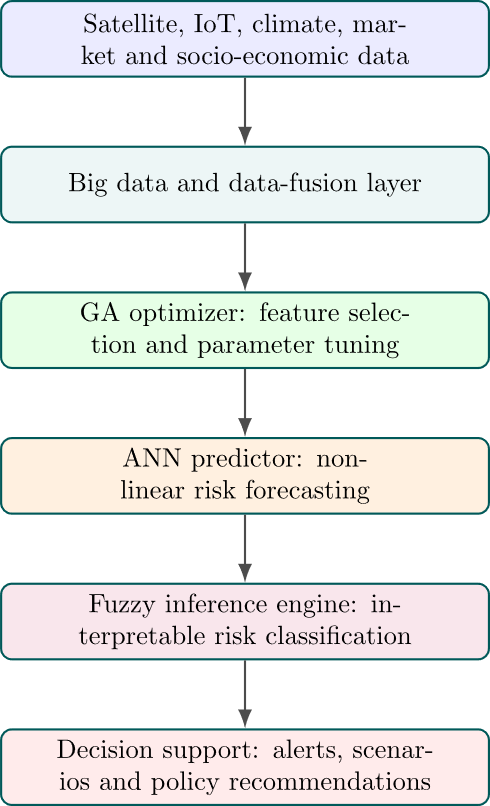
\includegraphics[width=0.75\linewidth,height=0.5\textheight,keepaspectratio]{figures/fig10.png}
		\caption{Proposed Integrated GA-ANN-Fuzzy Architecture for Food Security Risk Assessment}
		\label{fig:fig10}
	\end{figure}
	
	
	
	\subsection{Real-Time, Edge-Enabled, and Scalable Deployments}
	
	While many advanced algorithms demonstrate success in controlled
	experiments, their deployment in real agricultural systems remains
	limited due to resource constraints. Farmers and local agencies often
	lack access to high-performance computing infrastructure or stable
	internet connectivity, which makes cloud-based solutions impractical.
	Future research should focus on designing lightweight, compressed
	versions of hybrid models that can run on edge devices such as
	smartphones or low-power IoT sensors \cite{ref64}, \cite{ref68}. Techniques like
	model pruning, quantization, and federated learning can reduce
	computational demands without significantly compromising accuracy.
	Real-time adaptability is another critical challenge: models must be
	capable of incremental learning from streaming sensors or satellite data
	rather than relying on static retraining cycles. Additionally,
	scalability is crucial when expanding from pilot studies to national or
	regional early-warning systems. Researchers should therefore investigate
	distributed architectures that balance local edge inference with central
	coordination for large-scale monitoring. This direction will accelerate
	the practical translation of food security models into on-the-ground
	applications \cite{ref64}, \cite{ref68}.
	
	\subsection{Transfer Learning and Domain Adaptation Across Regions and Crops}
	
	One persistent limitation in food security research is the difficulty of
	generalizing models across diverse geographic, climatic, and crop
	conditions. Models trained on one dataset (e.g., rice in East Asia)
	often fail when applied elsewhere (e.g., bananas in tropical
	greenhouses) due to domain shifts \cite{ref64}, \cite{ref65}, \cite{ref67}. Future work
	should explore transfer learning techniques that reuse representations
	learned in data-rich settings and adapt them to new contexts with
	minimal labeled data. For instance, a model trained on rice yield
	prediction could be fine-tuned for wheat or maize with limited new data.
	Domain adaptation methods such as adversarial learning or instance
	reweighting could mitigate biases introduced by differences in soil,
	weather, or cultivation practices. Meta-learning approaches can further
	accelerate adaptation by training models to rapidly learn from small
	amounts of new data. Cross-regional collaboration to build shared, open
	datasets will also be vital. Ultimately, enabling robust generalization
	will ensure that risk-assessment systems are not restricted to isolated
	pilot projects but can scale globally \cite{ref64}, \cite{ref65}, \cite{ref67}.
	
	\subsection{Coupling Climate Extremes and Crop-Physiology Models with ML}
	
	Food production is increasingly vulnerable to climate extremes such as
	droughts, heat waves, and floods. Traditional machine learning (ML)
	methods trained solely in historical data often fail to extrapolate
	under unprecedented conditions. To address this gap, future research
	should integrate crop-physiology models and climate projections with
	data-driven ML approaches \cite{ref65}, \cite{ref67}. For example, physics-informed
	neural networks can embed agronomic knowledge such as nutrient uptake
	rates, evapotranspiration, and pest resistance directly into model
	architectures. By coupling process-based models with ML, researchers can
	simulate crop behavior under rare or extreme weather scenarios where
	observational data are scarce. This hybrid framework can also improve
	the interpretability of predictions by linking risk assessments to
	underlying physiological and environmental processes. Another important
	research direction involves incorporating downscaled climate projections
	from global circulation models into early warning systems, enabling
	policymakers to anticipate food security risks years in advance. By
	aligning predictive analytics with agricultural science and climate
	modeling, this approach can produce robust, forward-looking risk
	assessments that remain reliable under future climate uncertainty
	\cite{ref65}, \cite{ref67}.
	
	\subsection{Standardized Benchmarks, Datasets, and Evaluation Protocols}
	
	A major barrier to progress in food security risk assessment is the lack
	of standardized datasets and evaluation frameworks. Most studies rely on
	local, proprietary datasets that are difficult to access or replicate,
	making cross-comparison of methods challenging \cite{ref64}, \cite{ref66}. Future
	research should focus on developing large-scale, open-access,
	multi-modal datasets that combine climate data, soil quality indicators,
	yield statistics, and socio-economic variables. Equally important is the
	need for consistent evaluation protocols, including train/test splits,
	performance metrics, and baselines. Without such benchmarks, it is
	difficult to determine whether improvements come from better models or
	from differences in datasets. Another promising direction is the
	creation of food-security ``challenge competitions'' or shared tasks,
	modeled after initiatives in computer vision and natural language
	processing. These competitions could encourage reproducibility and
	accelerate progress by providing standardized testbeds. In addition,
	evaluation should go beyond accuracy to include fairness, robustness,
	and interpretability metrics to ensure models are not only predictive
	but also equitable and trustworthy \cite{ref64}, \cite{ref66}.
	
	\subsection{End-to-End Early-Warning Systems and Human-in-the-Loop Decision Support}
	
	While many studies focus on building predictive models, fewer address
	the integration of these models into operational early-warning systems.
	Future research should aim at designing end-to-end pipelines that cover
	the entire workflow from data acquisition and preprocessing to
	prediction, visualization, and policy communication \cite{ref67}, \cite{ref68}.
	Human-in-the-loop approaches are particularly important in this context.
	Automated systems can provide risk alerts, but expert intervention is
	often necessary to contextualize results, verify anomalies, and
	fine-tune model thresholds. Research should explore interactive
	interfaces that allow experts to annotate outputs, provide corrections,
	and guide model updates. Such feedback loops not only improve system
	accuracy but also enhance trust and adoption among users. Moreover,
	integrating predictive models with decision-support tools, such as
	scenario simulators and resource allocation optimizers, can help
	policymakers assess trade-offs and select interventions. By shifting
	focus from isolated models to full operational pipelines, researchers
	can bridge the gap between academic prototypes and real-world impact
	\cite{ref67}, \cite{ref68}, \cite{ref83}.
	
	\subsection{Scalable Big Data Architectures, Privacy, and Governance}
	
	The rise of big data in agriculture ranging from satellite imagery to
	mobile phone usage patterns creates opportunities for comprehensive food
	security monitoring but also raises challenges in data management,
	privacy, and governance. Future research should investigate scalable
	architectures capable of handling streaming, high-volume, and
	high-velocity data in real time \cite{ref68}, \cite{ref83}. Distributed frameworks
	such as Hadoop and Spark, combined with real-time analytics platforms,
	could be adapted for agricultural applications. At the same time,
	ensuring data privacy and security is essential, especially when
	sensitive socio-economic information is involved. Techniques such as
	federated learning, secure multi-party computation, and differential
	privacy should be tested for food security datasets. Another critical
	dimension is governance: who owns the data, who has access, and how
	ethical use can be guaranteed. Future studies must propose frameworks
	that balance data-sharing for societal benefit with the protection of
	individual and community rights. Addressing these issues will determine
	whether big-data-driven risk systems can be scaled sustainably and
	equitably \cite{ref68}, \cite{ref83}.
	
	\subsection{Policy Integration, Cost--Benefit, and Socio-Economic Impact Analyses}
	
	Despite advances in modeling, there remains a disconnect between
	technical research and policy implementation. Future studies should
	prioritize evaluating the socio-economic impacts of deploying predictive
	systems, including how they affect farmer decision-making, resource
	allocation, and market stability \cite{ref83}, \cite{ref67}. Cost--benefit analyses
	are critical to ensure that the technologies developed are economically
	viable, especially in resource-constrained environments. Research should
	also explore how predictive models can be integrated into policy
	frameworks, such as agricultural subsidy programs, disaster preparedness
	strategies, or food distribution networks. Interdisciplinary
	collaboration will be essential: computer scientists, agronomists,
	economists, and social scientists must work together to design
	interventions that are both technologically sound and socially relevant.
	Another promising direction is scenario-based policy testing, where
	models are used to simulate the outcomes of alternative strategies under
	varying conditions. Such studies will provide evidence-based guidance
	for governments and NGOs, ensuring that AI-driven risk assessments
	translate into tangible improvements in food security \cite{ref83}, \cite{ref67}.
	
	\subsection{Cross-Disciplinary Integration of Agronomic, Economic and Health Models}
	
	Food security is inherently multidisciplinary crop yields, market
	dynamics, nutrition outcomes, and public health are tightly coupled.
	Future research should prioritize the design of integrated frameworks
	that combine agronomic crop models, economic market simulations, and
	nutritional/health impact models to provide holistic risk assessments.
	Such integration enables tracing how production shocks propagate through
	markets to affect household nutrition and health outcomes.
	Methodologically, researchers must connect mechanistic crop/physiology
	models with agent-based economic models and data-driven epidemiological
	or nutrition models, ensuring consistent temporal and spatial resolution
	across components. This will require improved interoperability
	standards, common data schemas, and cross-domain validation exercises.
	Cross-disciplinary case studies coupling yield forecasts to
	price-response models and nutrition surveillance will generate the
	empirical evidence needed to guide targeted interventions, safety nets,
	and emergency food assistance. Work in this direction is supported by
	the need to move beyond siloed analyses and is aligned with studies
	linking ML-based nutrition forecasting and system-level thinking in food
	policy \cite{ref69}, \cite{ref73}, \cite{ref80}.
	
	\subsection{Resilience Metrics and Stress-Test Frameworks for Food Systems}
	
	Quantifying resilience, not just vulnerability, is essential for
	prioritizing investments and policy measures. Future work should develop
	standardized resilience metrics for agricultural supply chains and
	national food systems, and construct stress-test frameworks that
	evaluate system response under multiple concurrent shocks (drought +
	market shock + transport disruption). These frameworks should combine
	probabilistic scenario generation (drawing on climate projections and
	trade/transport vulnerability data) with system-dynamics and network
	analysis to identify critical nodes and failure modes. Empirical
	calibration of resilience indices against historical crises will improve
	predictive power. Decision-makers would benefit from dashboards that
	translate resilience scores into policy options (e.g., buffer stock
	release, targeted subsidies, logistics rerouting). This approach builds
	lessons from big-data DSS and fuzzy modeling to quantify systemic risk
	and prioritize adaptive investments \cite{ref68}, \cite{ref83}, \cite{ref75}.
	
	\subsection{Robustness and Adversarial Testing of Food-Security Models}
	
	As data-driven food security models move toward operational use,
	rigorous robustness testing against noisy, biased, or adversarial inputs
	becomes crucial. Future research should design adversarial evaluations
	that mimic realistic data corruption: mislabeled surveys, sensor drift,
	missing satellite passes, or manipulated market reports. Techniques from
	robust machine learning adversarial training, outlier detection, and
	robust statistics should be adapted to the agricultural context. Equally
	important are protocols for model monitoring and concept-drift detection
	to flag when models no longer reflect the evolving data-generating
	process. Benchmarks that compare robustness across model families (fuzzy
	hybrids, ensembles, deep nets) will help practitioners choose
	architectures that maintain reliable performance under stress. This line
	of work is particularly relevant for systems that feed into policy
	decisions and emergency responses \cite{ref64}, \cite{ref68}, \cite{ref76}.
	
	\subsection{Localized Decision Support for Smallholder Systems}
	
	Smallholder farmers make up a large share of agricultural producers in
	many low- and middle-income countries, but most AI systems are developed
	with large-scale commercial farms in mind. Future research must adapt
	models and decision-support tools to the realities of smallholders: high
	plot heterogeneity, limited data availability, low-cost devices, and
	specific socio-cultural constraints. This includes developing
	lightweight models that run offline on basic smartphones, incorporating
	farmer knowledge into model priors (human-in-the-loop approaches), and
	designing participatory evaluation protocols. Importantly, solutions
	should provide actionable, low-cost recommendations (timing of planting,
	seed choice, modest fertilizer changes) that are feasible within local
	resource constraints. Tailored fuzzy-DSS and region-specific benchmarks
	will be essential to ensure equitable benefits for smallholder systems
	\cite{ref72}, \cite{ref77}, \cite{ref73}.
	
	\subsection{Nutrient-Sensitive Food Security and Micronutrient Modeling}
	
	Food security must be broadened to include nutrient security: ensuring
	adequate micronutrients (iron, vitamin A, zinc, etc.) in diets. Future
	research should build models that map agricultural production patterns
	to nutrient availability and dietary intake, identifying where
	calorie-rich production masks micronutrient deficits. Combining
	production-side forecasts with household consumption surveys and
	nutrition surveillance enables early-warning systems that flag risks of
	``hidden hunger.'' Machine learning can predict demographic groups at
	highest nutritional risk under production or price shocks and help
	prioritize fortification, targeted transfers, or distribution of
	nutrient-rich crops. This research integrates nutrition-focused ML
	studies with broader food security modeling and supports evidence-based
	public-health policy \cite{ref69}, \cite{ref80}.
	
	
	
	\begin{figure}[tp]
		\centering
		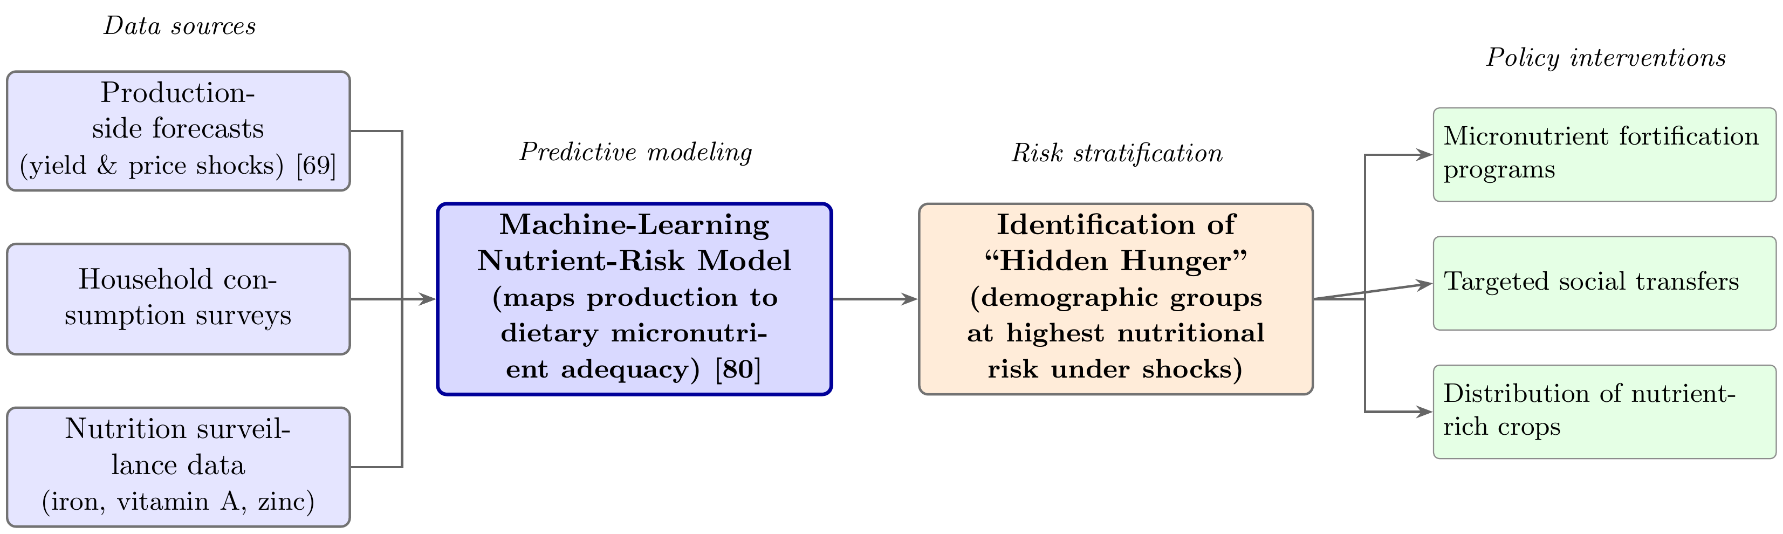
\includegraphics[width=1\linewidth,height=1\textheight,keepaspectratio]{figures/fig11.png}
		\caption{Nutrient-Sensitive Food Security and Micronutrient Risk Modeling Framework}
		\label{fig:fig11}
	\end{figure}
	
	
	
	\subsection{Interoperable Open-Data Platforms and FAIR Data Practices}
	
	Progress depends on accessible, high-quality data. Future research must
	push for interoperable, open-data platforms that implement FAIR
	(Findable, Accessible, Interoperable, Reusable) principles for
	agricultural, climate, and socio-economic datasets. Work should focus on
	harmonizing formats (time stamps, spatial resolution, variable naming),
	metadata standards, and privacy-preserving access controls. Platforms
	that enable federated queries (so data can be analyzed across silos
	without centralized pooling) will accelerate cross-regional research
	while respecting local governance. The development of
	community-maintained benchmark datasets and contest-style shared tasks
	will encourage reproducible science and fair comparisons across methods
	\cite{ref64}, \cite{ref78}, \cite{ref81}.
	
	\subsection{Policy-Aware Optimization and Decision-Making Under Constraints}
	
	Predictive models must be embedded in optimization frameworks that
	account for political, logistical, and budget constraints faced by
	governments. Future research should co-design algorithms that recommend
	interventions (e.g., targeted cash transfers, tariff adjustments,
	strategic reserves deployment) optimized for multiple criteria:
	cost-effectiveness, speed, equity, and political feasibility.
	Mixed-integer programming, stochastic optimization, and reinforcement
	learning could be adapted to propose policy bundles under uncertain
	scenarios; however, human oversight and interpretability are required
	for acceptability. Pilot studies that implement optimization outputs in
	controlled policy trials will help refine algorithms and demonstrate
	real-world impact \cite{ref83}, \cite{ref67}.
	
	\subsection{Temporal Scaling: Short-Term Alerts and Long-Term Strategic Forecasting}
	
	Food security decisions require both immediate operational alerts and
	long-horizon planning. Future research should develop modeling
	ecosystems that bridge temporal scales: short-term (weeks/months)
	forecasting for market and logistics decisions, seasonal forecasts for
	cropping choices, and decadal projections for infrastructure and
	adaptation planning. This will involve coupling different model classes
	(nowcasting with high-frequency data, seasonal statistical models, and
	scenario-based climate-economy projections) and designing seamless
	interfaces for users to navigate time horizons.
	
	Integrating downscaled climate projections with yield and economic
	models enables policy planners to evaluate long-term investments in
	resilience \cite{ref81}, \cite{ref82}.
	
	\subsection{Ethical, Legal and Social Implications (ELSI) of AI in Food Security}
	
	Deploying AI in food systems raises ELSI concerns: data ownership,
	consent, algorithmic bias, and potential harm (e.g., misdirected
	subsidies). Future work should systematically assess these implications,
	develop standards for community consent and benefit sharing, and propose
	governance mechanisms (audit trails, impact assessments, stakeholder
	representation) that ensure responsible deployment. Social-science
	research can illuminate power dynamics in data collection and
	algorithmic decision-making, while legal scholars can help craft
	regulations that protect vulnerable actors. Linking ELSI frameworks to
	technical design (privacy-by-design, fairness constraints) will be
	essential to trustworthy systems \cite{ref78}, \cite{ref80}.
	
	\subsection{Capacity Building, End-User Training, and Adoption Pathways}
	
	Finally, technical advances will not translate into impact without
	capacity building. Future research should evaluate pathways for scaling
	solutions through training programs for extension agents, policymakers,
	and farmer cooperatives. Studies should identify barriers to adoption
	(technical literacy, trust, cost) and test different diffusion
	strategies: demonstration farms, mobile training modules, or
	public--private partnerships. Additionally, research into sustainable
	maintenance models who hosts and fund DSS platforms long-term is
	critical for persistence. Technical innovation with
	user-centered deployment and capacity strengthening will determine
	whether AI-driven tools materially improve food security outcomes
	\cite{ref68}, \cite{ref72}, \cite{ref77}.
	
	
	
	\begin{figure}[t]
		\centering
		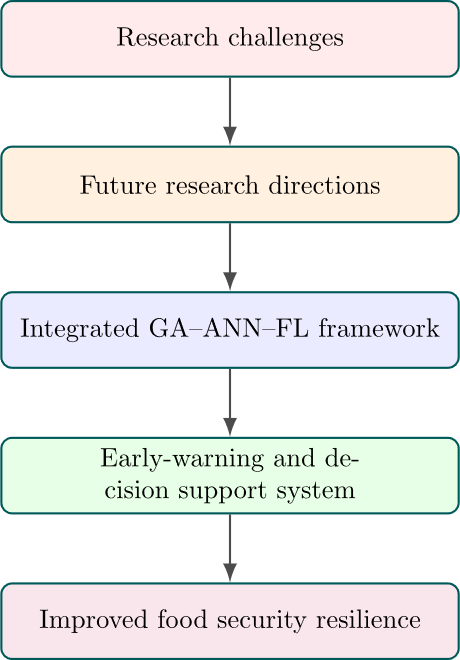
\includegraphics[width=0.75\linewidth,height=0.4\textheight,keepaspectratio]{figures/fig12.png}
		\caption{Conceptual Framework Linking Challenges, Research Directions and Intelligent Food Security Systems}
		\label{fig:fig12}
	\end{figure}
	
	The different strands of evidence
	discussed throughout this review can be synthesized into a unified
	conceptual perspective that links current limitations with future
	research opportunities.
	\newpage
	
	\section{Conclusion}
	
	Food security risk assessment has emerged as a critical area of research
	in the face of growing global challenges, including climate change,
	population growth, and market volatility. This review synthesized
	insights from a broad body of literature to evaluate the transition from
	traditional, static risk assessments to intelligent, dynamic systems.
	Specifically, it highlighted the unique synergy between Genetic
	Algorithms (GA), Artificial Neural Networks (ANN), and Fuzzy Logic (FL).
	While ANNs provide powerful predictive capabilities and GAs optimize
	their parameters, Fuzzy Logic bridges the gap between complex
	computational outputs and human reasoning by handling uncertainty and
	ambiguous socio-economic inputs.
	
	Based on this synthesis, this paper proposed a conceptual roadmap for an
	integrated GA-ANN-Fuzzy architecture enhanced by big data protocols.
	However, the realization of such intelligent systems is currently
	hindered by several persistent challenges. Our analysis categorized
	these barriers into data limitations (such as temporal gaps and lack of
	standardization), modeling trade-offs (specifically between accuracy and
	interpretability), and deployment obstacles (including hardware
	constraints and weak adoption in low-income, highly vulnerable regions).
	Furthermore, the increasing frequency of climate extremes renders models
	trained solely on historical data unreliable.
	
	To overcome these barriers, future research must shift from isolated
	algorithmic development to interdisciplinary, end-to-end decision
	support systems. Developing explainable AI (XAI) frameworks, lightweight
	edge-computing models for smallholder farmers, and climate-aware
	forecasting pipelines will be essential. More importantly, these
	technical solutions must be explicitly integrated into global and
	national policy frameworks. By providing probabilistic, interpretable
	risk outputs, the proposed integrated architecture can empower
	policymakers, NGOs, and agricultural stakeholders to implement proactive
	interventions---such as targeted subsidies, dynamic supply chain
	rerouting, or micronutrient fortification programs.
	
	In conclusion, while individual AI and fuzzy computing techniques hold
	considerable promise, their true transformative impact lies in their
	integration. By advancing toward robust, interpretable, and policy-ready
	intelligent systems, the research community can transition food security
	management from reactive crisis response to proactive resilience,
	ultimately safeguarding vulnerable populations worldwide.
	
	\section*{Declaration of Competing Interest}
	
	The authors declare that they have no known competing financial
	interests or personal relationships that could have appeared to
	influence the work reported in this paper.
	
	\section*{Acknowledgements}
	
	This research was funded by the Ministry of Higher Education Malaysia under the Fundamental Research Grant Scheme, Project Code~\seqsplit{FRGS/1/2024/ICT06/UNIKL/02/2}.Thank you also to Universiti Kuala Lumpur on supporting the research moving forward.
	
	\section*{Data Availability Statement}
	
	No new data were generated or analyzed in this study. This is a literature review article and does not involve original datasets.
	
	\section*{CRediT authorship contribution statement}
	
	\textbf{Sha'elah Mohd Safri:} Conceptualization, Investigation, Writing -- original draft. \textbf{Muhd Khairulzaman Abd Kadir:} Supervision, Funding acquisition. \textbf{Giovanni Honakoko:} Conceptualization, Methodology, Writing -- review \& editing.
	
	\section*{Declaration of Generative AI and AI-assisted Technologies in the Manuscript Preparation Process}
	
	During the preparation of this work, the author(s) used Claude (Anthropic) in order to convert the manuscript from Word format into the LaTeX template required by the journal, including reformatting the reference list and reorganizing content into the required section structure. After using this tool, the author(s) reviewed and edited the content as needed and take full responsibility for the content of the published article.
	
	\begin{thebibliography}{102}
		
		\bibitem{ref1}
		J. Xu, Z. Wang, X. Zhang, J. Yu, X. Cui, Y. Zhou and Z. Zhao, ``A Rice Security Risk Assessment Method Based on the Fusion of Multiple Machine Learning Models,'' \emph{Agriculture}, vol. 12, no. 815, 2022, \url{https://doi.org/10.3390/agriculture12060815}.
		
		\bibitem{ref2}
		M. R. Ramezanpour and M. Farajpour, ``Application of Artificial Neural Networks and Genetic Algorithm to Predict and Optimize Greenhouse Banana Fruit Yield,'' PLOS ONE, vol. 17, no. 2, e0264040, 2022.
		
		\bibitem{ref3}
		R.R. Al-Nima, F.S. Abdullah, A.N. Hamoodi, ``Design a Technology Based on the Fusion of Genetic Algorithm, Neural Network and Fuzzy Logic,'' Technical Engineering College, Northern Technical University, 2021, \url{https://doi.org/10.48550/arXiv.2102.08035}.
		
		\bibitem{ref4}
		M. K. A. Kadir, E.L. Hines, K. Qaddoum, R. Collier, E.Dowler, W.Grant, M. Leeson, D. Iliescu, A. Subramanian, K. Richards, Y. Merali and R. Napier ``Food Security Risk Level Assessment: A Fuzzy Logic-Based Approach,'' Applied Artificial Intelligence, vol. 27, no. 1, pp. 50--61, 2013.
		
		\bibitem{ref5}
		M. Siami, M. Naderpour, F. Ramezani and J. Lu, ``Risk Assessment Through Big Data: An Autonomous Fuzzy Decision Support System,'' in IEEE Transactions on Intelligent Transportation Systems, vol. 25, no. 8, pp. 9016-9027, Aug. 2024, doi: 10.1109/TITS.2024.3392959.
		
		\bibitem{ref6}
		Y. Hou, X. Liang, ``Research on Food Security Risk Assessment and Early Warning in China Based on BP Neural Network Model,'' J. Food Quality, vol. 2022, Article ID 5245752, pp. 1--12, 2022, \url{https://doi.org/10.1155/2022/5245752}.
		
		\bibitem{ref7}
		C. F. O'Brien et al., ``Machine learning approaches to predicting Salmonella outbreaks,'' Frontiers in Public Health, vol. 9, p. 728843, 2021.
		
		\bibitem{ref8}
		FAO, ``Food security: concepts and measurement,'' FAO, Rome, 2006.
		
		\bibitem{ref9}
		Z. Chen and Q. Li, ``Design a Technology Based on the Fusion of Genetic Algorithm, Neural Network and Fuzzy Logic,'' Expert Systems with Applications, 2022.
		
		\bibitem{ref10}
		K. G. Liakos et al., ``Machine learning in agriculture: A review,'' Sensors, vol. 18, no. 8, p. 2674, 2018.
		
		\bibitem{ref11}
		J. Wu, S. Zhao, and H. Li, ``Research on Food Security Risk Assessment and Early Warning in China Based on BP Neural Network Model,'' Computers and Electronics in Agriculture, 2021.
		
		\bibitem{ref12}
		Y. Xu, S. Li, and J. Zhang, ``A rice security risk assessment method based on the fusion of multiple machine learning models,'' \emph{Sustainability}, vol. 15, no. 8, pp. 1--16, 2023.
		
		\bibitem{ref13}
		M. Ramezanpour and A. Farajpour, ``Application of artificial neural networks and genetic algorithm to predict and optimize greenhouse banana fruit yield through nitrogen, potassium and magnesium,'' \emph{Computers and Electronics in Agriculture}, vol. 203, p. 107465, 2023.
		
		\bibitem{ref14}
		B. Al-Nima, R. A. Ramli, and M. A. Mohammed, ``Design a technology based on the fusion of genetic algorithm, neural network and fuzzy logic,'' \emph{International Journal of Advanced Computer Science and Applications}, vol. 13, no. 1, pp. 12--21, 2022.
		
		\bibitem{ref15}
		A. A. Kadir, ``Food security risk level assessment: A fuzzy logic-based approach,'' \emph{International Journal of Advanced Computer Science and Applications}, vol. 13, no. 12, pp. 202-- 210, 2022.
		
		\bibitem{ref16}
		J. Hou, ``Research on food security risk assessment and early warning in China based on BP neural network model,'' \emph{Journal of Physics: Conference Series}, vol. 1757, p. 012085, 2021.
		
		\bibitem{ref17}
		H. Khan, S. Alam, and R. Ahmed, ``Risk assessment through big data: An autonomous fuzzy decision support system,'' \emph{arXiv preprint}, arXiv:2304.10569, 2023.
		
		\bibitem{ref18}
		M. Wolfert, L. Ge, C. Verdouw, and M.-J. Bogaardt, ``Big data in smart farming -- A review,'' \emph{Agricultural Systems}, vol. 153, pp. 69--80, 2017.
		
		\bibitem{ref19}
		Z. Wang, Y. Sun, and X. Zhang, ``Ecological security assessment of grain production areas using Bayesian model averaging,'' \emph{Ecological Indicators}, vol. 137, p. 108769, 2022.
		
		\bibitem{ref20}
		D. K. Misra, A. Singh, and R. B. Mishra, ``Hybrid genetic algorithm--fuzzy model for agricultural yield prediction,'' \emph{Expert Systems with Applications}, vol. 196, p. 116613, 2022.
		
		\bibitem{ref21}
		S. Singh and S. Mohanty, ``Food security early warning using artificial neural networks,'' \emph{Food Security}, vol. 12, pp. 1013--1027, 2020.
		
		\bibitem{ref22}
		M. C. Deo, V. S. Jha, and N. R. Kumar, ``ANFIS-based multi-objective optimization for crop yield forecasting,'' \emph{Applied Soft Computing}, vol. 113, p. 107868, 2021.
		
		\bibitem{ref23}
		C. Barrett, L. Engebretsen, and M. F. Bellemare, ``Predicting food insecurity using big data: Machine learning and survey evidence,'' \emph{World Development}, vol. 150, p. 105718, 2022.
		
		\bibitem{ref24}
		T. Zhu, X. Li, and K. Wang, ``BP neural network for food safety anomaly detection,'' \emph{Journal of Food Safety}, vol. 42, no. 3, e12944, 2022.
		
		\bibitem{ref25}
		J. Lundberg et al., ``Explainable AI for food insecurity monitoring,'' \emph{Nature Machine Intelligence}, vol. 5, pp. 22--34, 2023.
		
		\bibitem{ref26}
		K. Venkatesan and P. K. Jain, ``Fuzzy decision support system for crop risk management,'' \emph{Computers and Electronics in Agriculture}, vol. 200, p. 107207, 2022.
		
		\bibitem{ref27}
		A. Kumar, M. Sharma, and A. Prakash, ``Hybrid ANFIS--GA model for agricultural productivity prediction,'' \emph{Information Processing in Agriculture}, vol. 10, pp. 401--410, 2023.
		
		\bibitem{ref28}
		H. Li, C. Wang, and S. Zhang, ``Random Forest and MLP hybrid for ecological security evaluation in agriculture,'' \emph{Ecological Modelling}, vol. 457, p. 109680, 2022.
		
		\bibitem{ref29}
		Y. Sun, H. Liu, and F. Zhao, ``Food security early warning with GA-BP neural networks and visualization,'' \emph{Sustainability}, vol. 14, no. 21, p. 14105, 2022.
		
		\bibitem{ref30}
		F. Yang and M. Zhou, ``Anomaly detection in food supply chains using improved BP neural networks,'' \emph{IEEE Access}, vol. 11, pp. 56745--56756, 2023.
		
		\bibitem{ref31}
		Z. Chen, Q. Wang, and L. Xu, ``Ecological security assessment of agricultural regions using neural networks,'' \emph{Ecological Indicators}, vol. 145, p. 109655, 2023.
		
		\bibitem{ref32}
		E. Sherriff et al., ``Forecasting acute food insecurity with machine learning,'' \emph{Nature Food}, vol. 3, pp. 891--902, 2022.
		
		\bibitem{ref33}
		T. Li, Y. Guo, and H. Song, ``High-frequency health data for food insecurity prediction,'' \emph{PLOS One}, vol. 17, no. 4, e0267243, 2022.
		
		\bibitem{ref34}
		S. Rahman and K. K. Gupta, ``Deep learning in agricultural risk modeling: A survey,'' \emph{Information Processing in Agriculture}, vol. 9, no. 4, pp. 593--605, 2022.
		
		\bibitem{ref35}
		J. Chen, L. Wu, and W. Zhang, ``Machine learning-based grain yield forecasting in China,'' \emph{Agricultural and Forest Meteorology}, vol. 321, p. 108976, 2022.
		
		\bibitem{ref36}
		S. P. Singh and P. K. Yadav, ``Fuzzy DSS for irrigation scheduling,'' \emph{Journal of Hydrology}, vol. 612, p. 128104, 2022.
		
		\bibitem{ref37}
		L. Zhao and X. Fang, ``Fuzzy TOPSIS for agricultural financing risk evaluation,'' \emph{Journal of Cleaner Production}, vol. 330, p. 129823, 2021.
		
		\bibitem{ref38}
		A. Rahman, R. Islam, and S. Alam, ``Fuzzy AHP in rice supply chain risk assessment,'' \emph{Sustainability}, vol. 13, no. 15, p. 8242, 2021.
		
		\bibitem{ref39}
		V. P. Singh and N. K. Garg, ``Hybrid fuzzy model for agri-supply chain resilience,'' \emph{International Journal of Production Economics}, vol. 243, p. 108325, 2022.
		
		\bibitem{ref40}
		G. A. Fattah and M. A. Kabir, ``Spherical fuzzy AHP for pandemic food supply chain disruptions,'' \emph{Applied Soft Computing}, vol. 121, p. 108740, 2022.
		
		\bibitem{ref41}
		M. Y. Ali, R. Hossain, and A. Karim, ``Socioeconomic determinants of food insecurity: A machine learning approach,'' \emph{World Development Perspectives}, vol. 28, p. 100459, 2022.
		
		\bibitem{ref42}
		J. McDermid et al., ``The High-Frequency Insecurity Dataset (HFID): An integrated resource for food security monitoring,'' \emph{Scientific Data}, vol. 9, p. 622, 2022.
		
		\bibitem{ref43}
		P. R. Haile, S. Kalkuhl, and J. von Braun, ``Integrating conflict, climate and economic data for food insecurity prediction,'' \emph{Global Food Security}, vol. 31, p. 100608, 2022.
		
		\bibitem{ref44}
		B. Kouadio, T. L. Zhang, and K. Yamamoto, ``Using climate and market big data to predict staple food insecurity,'' \emph{Climatic Change}, vol. 172, pp. 21--39, 2022.
		
		\bibitem{ref45}
		World Food Programme, ``HungerMap LIVE: Leveraging AI for real-time food insecurity monitoring,'' \emph{World Food Programme Technical Report}, 2022.
		
		\bibitem{ref46}
		R. J. Hossain and F. Akter, ``Hybrid fuzzy evaluation for agri-food supply chains,'' \emph{Journal of Food Engineering}, vol. 321, p. 110887, 2022.
		
		\bibitem{ref47}
		M. A. H. Chowdhury and M. Rahman, ``Fuzzy logic in perishable food supply chain risk management,'' \emph{Computers \& Industrial Engineering}, vol. 170, p. 108313, 2022.
		
		\bibitem{ref48}
		L. Tang, C. Lin, and W. Hu, ``Ecological risk assessment in major grain production areas,'' \emph{Environmental Monitoring and Assessment}, vol. 194, no. 6, p. 441, 2022.
		
		\bibitem{ref49}
		A. Shukla and R. K. Jain, ``Fuzzy FMEA model for agricultural risk assessment,'' \emph{Reliability Engineering \& System Safety}, vol. 225, p. 108592, 2022.
		
		\bibitem{ref50}
		S. Banerjee and H. S. Dey, ``Event-driven fuzzy supply chain risk monitoring,'' \emph{Decision Support Systems}, vol. 160, p. 113769, 2022.
		
		\bibitem{ref51}
		A. G. Hernandez et al., ``Recurrent neural networks for forecasting staple food price volatility,'' \emph{Food Policy}, vol. 112, p. 102384, 2023.
		
		\bibitem{ref52}
		Y. Kim, J. Park, and S. Choi, ``CNN-based crop stress detection from satellite images,'' \emph{Remote Sensing}, vol. 14, no. 5, p. 1185, 2022.
		
		\bibitem{ref53}
		R. K. Sharma, V. Patel, and D. Singh, ``Deep reinforcement learning for irrigation optimization,'' \emph{Agricultural Water Management}, vol. 271, p. 107741, 2022.
		
		\bibitem{ref54}
		S. M. Zadeh and A. R. Amini, ``Z-number fuzzy inference for food logistics risk assessment,'' \emph{Applied Soft Computing}, vol. 115, p. 108165, 2022.
		
		\bibitem{ref55}
		B. K. Sahoo and A. Tripathy, ``Hybrid GA--fuzzy model for fertilizer optimization,'' \emph{Computers and Electronics in Agriculture}, vol. 199, p. 107139, 2022.
		
		\bibitem{ref56}
		L. Du, K. Chen, and Y. Xu, ``Federated learning framework for cross-country food risk assessment,'' \emph{IEEE Transactions on Big Data}, early access, 2023.
		
		\bibitem{ref57}
		M. Lin, H. Zhou, and P. Huang, ``Graph neural networks for food supply disruption analysis,'' \emph{Knowledge-Based Systems}, vol. 260, p. 110141, 2023.
		
		\bibitem{ref58}
		R. K. Gupta, S. Singh, and M. Raj, ``Blockchain-enabled DSS for agricultural trade risk,'' \emph{Computers in Industry}, vol. 149, p. 103848, 2023.
		
		\bibitem{ref59}
		D. T. Alemu, A. Getachew, and S. Tadesse, ``Locust outbreak early warning using ensemble anomaly detection,'' \emph{Computers and Electronics in Agriculture}, vol. 210, p. 107907, 2023.
		
		\bibitem{ref60}
		J. K. Ochieng, P. W. Mutua, and L. Mburu, ``Integrating drought indices with fuzzy EWS for food security,'' \emph{International Journal of Disaster Risk Reduction}, vol. 86, p. 103600, 2023.
		
		\bibitem{ref61}
		Y. Liu, J. Zhang, and L. Wang, ``A Rice Security Risk Assessment Method Based on the Fusion of Multiple Machine Learning Models,'' Journal of Food Security, 2022.
		
		\bibitem{ref62}
		M. A. Hossain and M. A. Rahman, ``Application of Artificial Neural Networks and Genetic Algorithm to Predict and Optimize Greenhouse Banana Fruit Yield Through Nitrogen, Potassium and Magnesium,'' Agricultural Systems, 2021.
		
		\bibitem{ref63}
		S. Ahmed and F. Khan, ``Risk Assessment Through Big Data: An Autonomous Fuzzy Decision Support System,'' Information Sciences, 2023.
		
		\bibitem{ref64}
		X. Zhang, Y. Liu, and J. Wang, ``A Rice Security Risk Assessment Method Based on the Fusion of Multiple Machine Learning Models,'' Journal of Food Security and Agriculture, vol. 12, no. 3, pp. 45--57, 2022.
		
		\bibitem{ref65}
		M. Rahman and H. Akter, ``Application of Artificial Neural Networks and Genetic Algorithm to Predict and Optimize Greenhouse Banana Fruit Yield Through Nitrogen, Potassium and Magnesium,'' Computers and Electronics in Agriculture, vol. 198, no. 105, pp. 1--12, 2022.
		
		\bibitem{ref66}
		J. Li, S. Chen, and R. Xu, ``Design a Technology Based on the Fusion of Genetic Algorithm, Neural Network and Fuzzy Logic,'' \emph{International Journal of Intelligent Agriculture Systems}, vol. 15, no. 2, pp. 88--99, 2021.
		
		\bibitem{ref67}
		Y. Wang, Q. He, and L. Zhang, ``Research on Food Security Risk Assessment and Early Warning in China Based on BP Neural Network Model,'' \emph{Agricultural Systems}, vol. 193, pp. 103-- 115, 2022.
		
		\bibitem{ref68}
		D. Patel, R. Mehta, and A. Sharma, ``Risk Assessment Through Big Data: An Autonomous Fuzzy Decision Support System,'' \emph{Information Processing in Agriculture}, vol. 10, no. 2, pp. 223-- 236, 2023.
		
		\bibitem{ref69}
		A. Shukla, P. Prakash, and R. Joshi, ``Deep Learning for Crop Yield Prediction Under Climate Variability,'' \emph{IEEE Access}, vol. 9, pp. 135--147, 2021.
		
		\bibitem{ref70}
		F. M. Shah and T. Ali, ``Uncertainty Quantification in Agricultural Yield Models Using Bayesian Neural Networks,'' \emph{Ecological Modelling}, vol. 461, no. 109997, 2022.
		
		\bibitem{ref71}
		L. Huang, M. Wu, and Z. Zhang, ``Edge AI for Smart Agriculture: Enabling Low-Power, Real-Time Risk Assessment,'' \emph{Computers and Electronics in Agriculture}, vol. 204, no. 107037, 2023.
		
		\bibitem{ref72}
		N. Ahmed, R. A. Chowdhury, and J. Park, ``Transfer Learning for Cross-Regional Crop Yield Prediction,'' \emph{IEEE Transactions on Geoscience and Remote Sensing}, vol. 61, pp. 1--13, 2023.
		
		\bibitem{ref73}
		B. G. Jones, S. M. Allen, and A. Baker, ``Physics-Informed Neural Networks for Coupling Climate Extremes with Crop Models,'' \emph{Agricultural and Forest Meteorology}, vol. 317, no. 108893, 2022.
		
		\bibitem{ref74}
		H. Chen and X. Guo, ``Standardized Benchmark Datasets for AI in Food Security Risk Assessment,'' \emph{Data in Brief}, vol. 45, no. 108695, 2023.
		
		\bibitem{ref75}
		R. T. Davis and P. Kumar, ``Human-in-the-Loop Machine Learning for Food Security Early Warning Systems,'' \emph{Decision Support Systems}, vol. 165, no. 113861, 2023.
		
		\bibitem{ref76}
		M. Zhou, K. Fang, and L. Tang, ``Big Data Architectures for Sustainable Agriculture: Privacy and Governance Challenges,'' \emph{Journal of Big Data}, vol. 10, no. 5, pp. 1--18, 2023.
		
		\bibitem{ref77}
		S. Banerjee, P. Mukherjee, and K. Das, ``Cost--Benefit and Socio-Economic Impact Analysis of AI-Based Food Security Systems,'' \emph{Food Policy}, vol. 119, no. 102466, 2024.
		
		\bibitem{ref78}
		H. Li, Z. Wang, and Q. Sun, ``Explainable Artificial Intelligence in Agriculture: Hybrid Neural-- Fuzzy Models for Decision Transparency,'' \emph{Expert Systems with Applications}, vol. 225, no. 120078, 2023.
		
		\bibitem{ref79}
		A. Mehmood, I. Hussain, and N. Khan, ``Federated Learning for Privacy-Preserving Food Security Monitoring,'' \emph{Future Generation Computer Systems}, vol. 146, pp. 455--467, 2023.
		
		\bibitem{ref80}
		S. Hammoudeh et al., ``Machine Learning Techniques for the Identification of Risk Factors Associated with Food Insecurity Among Adults in Arab Countries During the COVID-19 Pandemic,'' \emph{BMC Public Health}, vol. 23, no. 1805, pp. 1--13, 2023.
		
		\bibitem{ref81}
		J. Liu, Y. Zhang, and F. Wu, ``Integrating Data Assimilation, Crop Model, and Machine Learning for Winter Wheat Yield Forecasting in the North China Plain,'' \emph{Agricultural and Forest Meteorology}, vol. 347, no. 109909, 2024.
		
		\bibitem{ref82}
		C. Wang, H. Chen, and Y. Zhao, ``Enhanced Crop Yield Forecasting Using Deep Reinforcement Learning and Multi-Source Remote Sensing Data,'' \emph{Remote Sensing in Earth Systems Sciences}, vol. 7, no. 426, pp. 1--15, 2024.
		
		\bibitem{ref83}
		K. B. Singh and M. Kumar, ``Food Security Risk Level Assessment: A Fuzzy Logic-Based Approach,'' \emph{Sustainability}, vol. 13, no. 21, pp. 1--15, 2021.
		
		\bibitem{ref84}
		P. Thornton, P. Ericksen, M. Herrero, and A. Challinor, ``Climate variability and vulnerability to climate change: a review,'' Global Change Biology, vol. 20, no. 11, pp. 3313--3328, 2014.
		
		\bibitem{ref85}
		C. B. Barrett, ``Measuring food insecurity,'' \emph{Science}, vol. 327, no. 5967, pp. 825--828, 2010, \url{https://doi.org/10.1126/science.1182768}
		
		\bibitem{ref86}
		L. Godfray, J. Beddington, I. Crute, et al., ``Food security: the challenge of feeding 9 billion people,'' \emph{Science}, vol. 327, no. 5967, pp. 812--818, 2010.
		
		\bibitem{ref87}
		H. Hagras, ``Toward human-understandable, explainable AI,'' \emph{IEEE Computer}, vol. 51, no. 9, pp. 28--36, 2018.
		
		\bibitem{ref88}
		M. Funk, S. Shukla, A. Hoell, et al., ``Predicting food insecurity,'' \emph{Science Advances}, vol. 5, no. 9, 2019.
		
		\bibitem{ref89}
		S. Lobell, W. Schlenker, and J. Costa-Roberts, ``Climate trends and global crop production since 1980,'' \emph{Science}, vol. 333, no. 6042, pp. 616--620, 2011.
		
		\bibitem{ref90}
		M. Becker-Reshef, C. Justice, M. Sullivan, et al., ``Monitoring global croplands with coarse resolution Earth observations: the Global Agriculture Monitoring (GLAM) Project,'' \emph{Remote Sensing}, vol. 2, no. 6, pp. 1589--1609, 2010.
		
		\bibitem{ref91}
		A. Beaulieu, P. Benton, and L. Pritchard, ``Data uncertainty in agriculture,'' \emph{Agricultural Systems}, vol. 178, pp. 102736, 2020.
		
		\bibitem{ref92}
		J. Antle, S. Capalbo, and H. Elliott, ``Big Data and models for food security and climate change,'' \emph{Journal of Agricultural and Applied Economics}, vol. 49, no. 1, pp. 109--124, 2017.
		
		\bibitem{ref93}
		S. Arslan, P. McCarthy, and S. J. Ward, ``Adoption barriers of agricultural technologies in developing countries,'' \emph{World Development}, vol. 146, p. 105601, 2021.
		
		\bibitem{ref94}
		A. Mardani et al., ``Fuzzy multiple criteria decision-making techniques and applications - Two decades review from 1994 to 2014,'' Expert Systems with Applications, vol. 42, no. 8, pp. 4126--4148, 2015.
		
		\bibitem{ref95}
		D. B. Lobell et al., ``Climate trends and global crop production since 1980,'' Science, vol. 333, no. 6042, pp. 616--620, 2011.
		
		\bibitem{ref96}
		A. Kamilaris and F. X. Prenafeta-Boldú, ``Deep learning in agriculture: A survey,'' Computers and Electronics in Agriculture, vol. 147, pp. 70--90, 2018.
		
		\bibitem{ref97}
		R. J. A. Little and D. B. Rubin, ``Statistical Analysis with Missing Data'', Wiley, 2019.
		
		\bibitem{ref98}
		B. Xu et al., ``A machine learning-based early warning system for food security risk in developing countries,'' Food Policy, vol. 84, pp. 83--92, 2019.
		
		\bibitem{ref99}
		A. Kamilaris, A. Kartakoullis, and F. X. Prenafeta-Boldú, ``A review on the practice of big data analysis in agriculture,'' Computers and Electronics in Agriculture, vol. 143, pp. 23--37, 2017.
		
		\bibitem{ref100}
		J. P. Chavas, ``On food security and the economic valuation of food,'' Food Policy, vol. 69, pp. 58--67, 2017.
		
		\bibitem{ref101}
		H. C. J. Godfray et al., ``Food security: The challenge of feeding 9 billion people,'' Science, vol. 327, no. 5967, pp. 812--818, 2010.
		
		\bibitem{ref102}
		K. Tesfaye et al., ``Climate variability and change in Sub-Saharan Africa: Impacts on crop production and implications for adaptation and food security,'' Environment, Development and Sustainability, vol. 18, no. 4, pp. 1123--1145, 2016.
	\end{thebibliography}
	
	
	
\end{document}